
\documentclass[promaster]{thesis-uestc}

\title{面向数据价值共享的激励机制设计与实现}{An Incentive Mechanism for Data Sharing}

\author{罗通}{Luo Tong}
\advisor{罗光春\chinesespace 教授}{Dr. Guangchun Luo}
\school{计算机科学与工程学院\chineseleftparenthesis网络空间安全学院\chineserightparenthesis}{School of Computer Science and Engineering}
\major{计算机技术}{Computer Technology}
\studentnumber{201722060929}

\begin{document}

\makecover

\begin{chineseabstract}
为了适应日益增长的宽带信号和非线性系统的工程应用,用于分析瞬态电磁散射问题的时域积分方程方法研究日趋活跃。本文以时域积分方程时间步进算法及其快速算法为研究课题,重点研究了时间步进算法的数值实现技术、后时稳定性问题以及两层平面波算法加速计算等,主要研究内容分为四部分。

……

\chinesekeyword{时域电磁散射,时域积分方程,时间步进算法,后时不稳定性,时域平面波算法}
\end{chineseabstract}

\begin{englishabstract}
With the widespread engineering applications ranging from broadband signals and non-linear systems, time-domain integral equations (TDIE) methods for analyzing transient electromagnetic scattering problems are becoming widely used nowadays. TDIE-based marching-on-in-time (MOT) scheme and its fast algorithm are researched in this dissertation, including the numerical techniques of MOT scheme, late-time stability of MOT scheme, and two-level PWTD-enhanced MOT scheme. The contents are divided into four parts shown as follows.

\englishkeyword{time-domain electromagnetic scattering, time-domain integral equation (TDIE), marching-on in-time (MOT) scheme, late-time instability, plane wave time-domain (PWTD) algorithm}
\end{englishabstract}

\thesistableofcontents

\thesischapterexordium

\section{研究工作的背景与意义}

在科学技术不断发展的今天,人类的一切活动及其产生的影响都可以被信息化。衣食住行、自然观测、历史记载等领域都不例外。随之产生的海量数据中存在巨大的潜在价值,现在已经有精彩纷呈的数据挖掘及分析技术(机器学习、深度学习等)应用于这些数据上,训练网络、学习知识,从而获取巨大的社会及经济价值。《2019中国大数据产业发展白皮书》\cite{2019baipishu}指出,2015年以来,随着国家和地方政府的大力推动,大数据产业加速发展。2018年整体规模达到4384.5亿元,预计到2021年将达到8070.6亿元,持续促进传统产业转型升级,激发经济增长活力,主力新型智慧城市和数字化建设。海量数据早已成为一种重要的资源。然而在数据的使用方法不断革新,前途一片光明的同时,数据使用的合法性、安全性也成为亟待解决的难题。各个数据拥有者,可能出于隐私防护、利益诉求、知识产权、保密责任等各种原因,不愿将数据共享,以创造更大的价值。于是,各个“数据孤岛”产生了。而在网络安全事件,隐私泄露事件频发的今天,面对复杂的低信任度网络环境,如何打破这些孤岛之间的共享障碍,促进数据的价值更好得流通,同时限制数据暴露的程度来降低数据安全风险是现有研究努力的方向。

%“大数据”指的数据规模太大或者复杂以至于无法以传统方式进行处理。具有三个方面的特征:
%1、规模:各个机构组织从不同来源进行数据收集:包括商业交易,智能设备(IOT),工业设施,电子音像、社会媒体等等。在过去,存储这些数据也是极大的难题。
%2、速度:随着物联网的快速发展,商业中的数据流必须。

另一方面,数据价值的共享必然不可避免得带给数据拥有者损失,这不利于数据拥有者主动参与价值共享生态。这要求系统对数据拥有者进行补偿,从而鼓励数据拥有者在受限的数据暴露程度下贡献其数据价值。系统中的环境、规则形成了整个数据价值共享的体系机制,好的规则体系能够充分调动所有数据拥有方的积极性,提升整体性能。而坏的机制可能使得数据拥有者罢工,为体系带来一系列不可估量的风险,甚至使整个系统停止运转。因而在打破“数据孤岛”壁垒的同时,针对具体应用场景确定性能优良的价格体系,完善激励机制对数据价值共享生态有着极大的促进和支撑作用。但大数据产业目前仍然处于探索与研究的阶段,机制体系等基础设施并不完善。针对潜在的新数据价值共享模式设计公平合理、计算高效的价格体系是具有重要意义的。


\section{国内外研究历史与现状}

占有策略激励相容的概念是由Hurwicz\citing{hurwicz1972informationally}在1972年正式提出。而理想机制的概念起源于Vickrey\citing{vickrey1961counterspeculation},这篇文章也是拍卖理论的奠基之作。搜索引擎的主要收入来源是关键字拍卖,关键字拍卖的广义二价拍卖(GSP)模型模型来源于Edelman\citing{edelman2007internet}和Varian\citing{varian2007position}。而拍卖者具有指定税收目标的拍卖机制由Goldberg等人\citing{goldberg2006competitive}讨论及分析。

另一方面,算法机制设计起源于Nisan\citing{nisan2001algorithmic}和Lehmann等人\citing{lehmann2002truth}。单变量环境的概念由Archer和Tardos\citing{archer2001truthful}于2001年提出。而在资源分配领域应用广泛的背包拍卖是由Mu'Alem和Nisan\citing{mu2008truthful}提出。显示定理来自于Gibbard\citing{gibbard1973manipulation}。而近年来算法机制设计领域的快速发展得益于其与近似算法领域的紧密连接。Ibarra和Kim\citing{ibarra1975fast}于1975年给出了背包问题的经典FPTAS近似算法。Briest\citing{briest2005approximation}以此为基础给出了计算可行且性质良好的背包拍卖机制。类似的,Lehmann等人\citing{lehmann2002truth}以集合覆盖问题为基础,以贪心算法实现了性质良好的机制。

前述的算法大多考虑社会福利最大化,而着重考虑拍卖方收益的最优拍卖机制起源于Myerson\citing{myerson1981optimal}的研究。Ostrovsky和Schwarz\citing{ostrovsky2009reserve}在将此思想应用至雅虎公司的关键字拍卖中。雅虎高层管理者认为设置更高的保留价格是雅虎公司在2008年第三季度的搜索引擎获利增加的最主要原因。

机制设计的应用场景还涉及频谱拍卖领域。在单次频谱拍卖中,可能涉及的金额高达百万美元。因而失败的机制将带来不可挽回的经济损失。Rassenti等人\citing{rassenti1982combinatorial}早在1982年就尝试以组合拍卖来确定机场的时隙分配。Cramon\citing{cramton2000collusive}详细描述了早期频谱拍卖中的出现的共谋和竞标信号问题。美国联邦通信委员会(FCC)\citing{federal2015procedures}于2015年给出了FCC激励拍卖机制的细节。该机制使政府可以以反向拍卖的方式从广播电视台回购频谱,同时保证未被回购的频谱不会产生冲突,然后进行资源整合并重新出售整合后的宽频谱,从而更好得分配频谱资源并带来更多的经济收益。其反向拍卖的核心问题与平面图的点着色问题有关。

前述的机制及算法大都是以货币作为激励手段,另一种无货币的机制也有重要应用场景。Roth等人\citing{roth2004kidney}以TTC算法来解决肾脏交换的问题。但TTC算法的结果可能包含较长的置换链,这增加了肾脏交换过程中的风险。因此其将原问题建模为无向图,并通过图的匹配来寻找长度仅为2的置换链\cite{roth2005pairwise}。另外,Roth在\cite{roth2004kidney}还将TTC算法及其激励特性应用至所有人亡故的房屋与没有住所的人的匹配问题。而在\cite{roth2007efficient}中,Roth等人进一步考虑置换链长度为3的肾脏匹配机制,这意味着同时进行6个患者的手术。相比于长度为2的置换链,这极大提升了肾脏匹配成功的数量。但是,继续增大置换链的长度,例如4、5,以至更长,似乎都难以显著提升匹配数量。Sack\citing{sack201260}在2012年实施了一场置换链长度为30的肾脏移植,由一名无偿肾源捐献者作为置换链的起点。前述算法的激励层级大多是在患者级别,即每个患者尽表达尽可能多的肾脏交换意愿是其占有策略,这有利于促成更多的成功匹配。然而,若在肾脏交换意愿在医院层面被部分拦截,即医院内部尽可能最优匹配,这可能不利于总体系统的匹配性能。这部分其实与共谋有关。Ashlagi等人\citing{ashlagi2015mix}针对肾脏置换场景下医院层面的激励机制做了一些关于讨论。

另外一个应用场景是稳定匹配问题。Gale和Shapley\citing{gale1962college}形式化了稳定匹配问题,给出了延迟接受算法,并证明了是算法的时间复杂度和部分最优性。Dubins和Freedman\citing{dubins1981machiavelli}研究了上述场景的一个变种:未匹配的参与者希望依次进行匹配而非同时进行。他们还分析证明了延迟接受算法的激励属性:算法对匹配的一方具有真实表达意愿的激励,而对另一方没有。

最近的激励机制的相关应用主要集中在众包领域、频谱拍卖\cite{gao2010map}\cite{wang2011district}\cite{yang2014promise}\cite{zhou2008ebay}、路由\cite{zhong2007designing}、协同通信\cite{chen2010conflicts}\cite{yang2011truthful}等。此处以与数据价值共享有关的众包领域为例。$SenseMart$\cite{chou2007sensing}讨论了在感知数据交付机制中的激励问题并提出了一系列更具有挑战的难题。另外在众包与相近的参与感知领域中也存在一些关于激励机制的研究。Reddy等人\citing{reddy2010recruitment}来设计了一种匹配关于感知任务的最优参与者的激励框架。然而,他们仅仅关注于参与者的选择,而并未涉及激励机制的设计。Danezis等人\citing{danezis2005much}设计了一种密封二价拍卖机制来提高参与者的参与度。然而,他们没有在机制设计中进一步考虑众包者本身的效用。Lee和Hoh\citing{lee2010sell}设计并且评估了一种动态价格激励机制,参与者可以将感知数据以自己的标的价格卖给需求方,但这种机制中的参与者可能会为了最大化自身效用而给出非真实估值。duan等人\citing{duan2012incentive}研究了两种应用场景:数据获取和分布式计算。对于数据获取,他们考虑了一种阈值模型来保证数据感知的有效性,并且所有的参与者共享预设的报酬。对于分布式计算的场景,他们设计了一种基于契约理论的机制来适应参与者的多样性。另外Li和Cao\citing{li2013providing}在激励机制设计中考虑了隐私保护的目标。另外,还有存在一些特殊目的机制设计。Koutsopoulos\citing{koutsopoulos2013optimal}研究了一种随机化的激励机制,在保证能够达到某一阈值的数据感知服务质量级别的情况下,最小化付给参与者的报酬。在参与者估值的概率分布已知的情况下,Luo等人\citing{luo2014profit}设计了一种最大化期望收益同时满足理性人约束的激励体系。这些提及的机制均为离线机制,即众包者获取所有的信息后再进行参与者选择。而一些在线机制也有被研究与讨论,Zhao等人\citing{zhao2014crowdsource}就设计了在线的激励机制,每个参与者到达时,众包者必须就现有信息立即给出该参与者的胜出结果。



\section{本文的研究目标与研究内容}
由相关领域的研究历史及现状可知,激励机制已经被应用于科学与应用的诸多方面。但是在数据价值共享领域,面向潜在的数据共享模式的激励机制是缺乏的。因而本文给出一种理想的分布式计算模式——多方数据价值共享计算,然后以此为基础,挖掘数据共享流程中的细节信息,并设计不同应用场景中的激励机制,鼓励“数据孤岛”之间互联互通,在受限的数据暴露程度下使用数据,充分创造新的价值。确切的说,主要有以下三个研究点:
\begin{enumerate}
    \item 分析多方计算的简单可并行场景的特点及限制,对问题进行形式化建模,应用拍卖理论,设计一种具有计算有效、真实、社会福利最大等优秀性质的激励机制。
    \item 从计算依赖相关的多方计算场景出发,对问题进行形式化建模,深入剖析,设计一种具有计算有效、真实、社会福利最大等优良性质的机制。同时给出该场景下的最优机制的设计。实施模拟实验对算法性能进行论证分析。
    \item 实现数据价值共享系统,将上述算法机制进行实装,验证其有效性。
\end{enumerate}


\section{本论文的结构安排}
本文的章节结构安排如下:

第一章,分析本文的研究背景和研究意义,论述本题相关领域的算法及应用的国内外研究历史和现状。确定本文的研究目标与研究内容,最后对全文章节结构进行梳理。

第二章,介绍本文用到的相关理论。主要是算法机制设计和拍卖理论。

第三章,介绍新的数据价值共享计算模式——多方计算。针对简单可并行的具体计算场景做机制设计。共有三个子问题:1、无特殊限制的简单可并行计算基础拍卖模型。2、多重指标限制模型。3、树形机构关系模型。每个子问题均进行形式化建模、分析、求解。

第四章,研究计算依赖相关的机制设计问题。考虑时效性限制在该场景下的重要影响,对问题进行详尽的论述分析。然后设计该场景下的最优机制。最后,进行模拟实验,并论述算法的有效性和准确性。

第五章,实现数据价值共享系统,将上述算法部署至应用环境。给出总体设计、模块设计、及测试分析。最后对应用系统的功能界面进行展示。

第六章,对全文进行总结陈述,分析本文的工作可取之处与不足,并展望后续工作的可能研究方向。

\section{本章小结}
本章分析了本文研究背景、意义。论述了算法机制设计的部分历史来源及其在频谱拍卖、众包、医疗卫生等领域的不同应用现状,并确定了全文的研究内容和目标。最后梳理了全文结构。


\chapter{相关理论基础}
本章介绍后文涉及的相关理论及技术,主要是算法机制设计与拍卖理论。只有在这些理论基础上才能结合具体场景,设计性质良好的激励机制。

\section{机制设计}
在日常生活中,我们会遇到许多需要策略决策的场景,例如我们需要卖出一台二手电视机,但我们并不知道应该为其确定怎样的合适价格。又或者我们需要确定在办公室购置一台新的电冰箱,而我们并不知道同事们愿意为这个冰箱各自付出多少经济支持。我们可能会依次去询问他们,并告诉后面的人前面的人的估值。也可以同时询问所有人的估值来判断是否购入冰箱。当然,两种模式产生的效果是不同的。这两种模式都在参与者中引入了一种非合作性的策略博弈。参与者知道博弈的结果不仅取决于自身的选择,也取决于其他人的策略。因而每个参与者自身的最优策略依赖于其他参与者的策略。机制设计理论因此建立于博弈论。博弈论以游戏的规作为输入,对策略玩家的表现进行预测。而机制设计是关于选择游戏的最优规则。更确切得说,机制设计是关于多个参与者的隐藏信息,在二手电视机的问题中,它是各个买家参与者对这台电视机的内心真实估值。而在冰箱问题中,它是同事对新冰箱的真实购买意愿。机制规则一旦被确定后,便不再更改,无论是参与者还是设计者。这是机制有效运行的基础。
\subsection{简单拍卖及理想机制}
\subsubsection{单物品拍卖}
考虑现有一个卖家,仅有一件物品需要卖出。同时有$n$个潜在的买家需要购买该物品。为了对买家的策略进行推断,我们需要一个模型来描述买家的收益。第一个关键假设是每个买家都有一个非负的估值$v_i$,来表征他对该物品的真实购买需求程度。在现实场景中,人的真实购买需求意愿是不断变化的。但在此模型中,对于每个买方,其真实估值$v_i$被认为是不变且私密的,即除了该买家自己,卖方和其它买方都无法获得其真实值。买家的效用函数模型为:$u_i$ = $v_i-p_i$,若买家获得该物品;$0$,若买家未获得。这被称为准线性效用模型,本文也采用该模型来描述各个参与者的效用。
\subsubsection{最高价拍卖}
对于单物品拍卖,其流程大致是:

\begin{enumerate}
    \item 买方给出密封标的$b_i$
    \item 确定胜出者,并将物品分配给胜出者。
    \item 买方向卖方支付价格$p_i$
\end{enumerate} 

其中,第二步的最简单实现是直接将物品分配给标的最高的买方。而第三步价格的确定,可以有多种选择,例如直接向卖方支付胜出者的标的价格(称为最高价拍卖),或者次高价格,亦或是直接令支付价格为0。在不同的价格机制下,买方都会制定相应的标的策略来使自己的效益最大化。因而买方的行为及拍卖的结果都会随着价格机制的变化而变化。

最高价拍卖是常见的拍卖类型,在许多藏品流通、地产交易等市场均有广泛的应用。然而最高价拍卖,尤其是密封拍卖,是一种难以分析推理的拍卖模式。作为一个参与者,在准线性效用下,难以找到使自身收益最大的标的策略。因为在直接显示的机制下,无论参与者是胜出还是失败,其效用均为0。相应的,作为一个卖方,或者是机制设计者,很难预测系统的整体局面及结果。

\subsubsection{二价拍卖与占优策略}
 另一种同样应用广泛且极其重要的拍卖机制是二价拍卖,也称Vickery拍卖。其实一种密封拍卖机制:最高标的者作为胜出者获得物品的分配,并向卖方支付除其自身标的以外的最高标的价格。为了描述这种拍卖机制的优良性质,此处给出占优策略的简单定义。
 \begin{definition}[占优策略]
     无论其他参与者如何投标,该参与者的一种策略(即标的),都能够最大化其效用。
 \end{definition}
 于是,二价拍卖的激励特点如下所示。
 \begin{corollary}[二价拍卖中的激励]
     在二价拍卖机制中,每个参与者$i$都有一个占优策略:使标的$bid_i$等于其对物品的真实估值$v_i$。
 \end{corollary}
二价拍卖的另一个重要特点是,一个真实表达估值的参与者不会在二价拍卖中受损。这可以鼓励更多的真实表达的参与者加入到拍卖环节中。该特点也被称为个人理性约束。
\begin{corollary}[效用非负性]
    在二价拍卖机制中,每个真实投标的参与者都能够保证其效用非负。
\end{corollary}
\subsubsection{理想机制}
从二价拍卖中可以归纳总结出性质良好的机制的特点,应用至更加广泛的机制设计中。首先,给出相关概念的定义。
\begin{definition}[占优策略激励相容(Dominant-Strategy incentive Compatible)]
    在一个机制中,若对每个参与者来说,真实的投标总是其占优策略,并且任意真实投标的参与者总能获得非负的效用。那么这个机制被称为具有占优策略激励相容的特性。
\end{definition}

然后是拍卖中关于社会福利的定义。这个概念体现了拍卖机制的有效性及积极意义,若最大化社会福利对应着将物品分配给真正需要的人。
\begin{definition}[社会福利]
    单物品拍卖中的社会福利定义为:$\sum_{i=1}^{n}{v_ix_i}$,若参与者$i$胜出,则$x_i=1$,否则$x_i=0$。
\end{definition}

由前述的定义可以得出理想机制的特点,这也是本文需要着重研究设计的激励机制特性。
\begin{enumerate}
    \item \textbf{强激励保证}:该机制满足占优策略激励相容$(DSIC)$
    \item  \textbf{有效性保证}:该机制满足社会福利最大化
    \item \textbf{计算有效性保证}:该机制可以在多项式时间内实现
\end{enumerate}
这三种性质都是极为重要的。从参与者的角度来说,DSIC的特性使得其可以很容易的选择标的来参与到机制中。这泯灭了有高级参与者和初级参与者之间的经验差异。从卖方或者是机制设计者的角度来看,DSIC的机制特性使得推断机制的结果局面变得更为容易可行。值得一提的是,任何机制局面的推断都依赖于对参与者行为的假设。在一个DSIC的拍卖机制中,仅有的假设是参与者以占优策略参与到拍卖环节。这是一个关于参与者行为的弱假设。这也符合真实的理性人的一般行为,有利于设计研究的激励机制应用到真实应用场景并取得较优的性能结果。
DSIC特性是值得采纳和研究的,然而DSIC的机制设计空间仍然较大。例如,一个随机赠予的拍卖机制也符合DSIC的特性。因为,参与者给出的非真实标的无法增加其获胜的可能性。然而,分配规则一旦不依赖于参与者的标的,会造成机制的有效性丧失,无法提升系统整体性能。此时,社会福利最大的特性就显得尤其重要。二价拍卖机制在解决社会福利最大的同时,保证了DSIC的性质,并在线性时间复杂度内求解。因而其是一种性质优秀的理想机制典型。

\subsection{麦尔森引理}
\subsubsection{单变量环境}
如前文所述,机制设计关注的是参与者自身的隐藏信息。而以隐藏信息做分类,可以将机制设计的情形划分为单变量环境与多变量环境。直观上来讲,单变量环境指的是各个参与者的私密信息是单个值。在单变量环境中,麦尔森引理是确定价格的有力工具,而与多变量环境相对应的是VCG机制。
\subsubsection{引理表述}
一个机制以参与者的标的$\mathbf{b}$作为输入,然后确定胜出者及相应的分配$\mathbf{x}$,$x_i$是分配给参与者$i$的物品数量。最后确定需要支付的价格$\mathbf{p}$,$p_i$是参与者$i$的价格。而单变量环境下DSIC机制的设计可以简单的归纳为对分配规则$\mathbf{x(b)}$和价格规则$\mathbf{p(b)}$的确定,保证激励机制的有效性。
麦尔森引理确定了机制的分配函数与价格函数之间的数量关系。然而并非所有分配函数都可以设计为拥有前述优良性质的激励机制。首先给出关于分配函数的两个定义。
\begin{definition}[可实施的分配规则]
一个分配规则$\mathbf{x}$是可实施的,当且仅当存在一个价格规则$\mathbf{p}$,使得直接显示机制$(x,p)$满足DSIC的性质。
\end{definition}
由上述定义可知,可实施的分配规则是那些可以扩展为DSIC机制的分配规则。等价地说,DSIC机制在分配规则上的投影也满足可实施的性质。若我们的设计目标是一个DSIC的机制,那么我们需要限制在可实施的分配规则这个集合内。这相当于是我们机制设计的可行集。

\begin{definition}[单调分配规则]
    单变量环境下的一个分配规则$x$被称为是单调的,当且仅当对于任意参与者$i$以及任意$\mathbf{b_{-i}}$\footnote{表示除$bid_i$分量以外的总标的向量},分配规则$x_i(z,\mathbf{b_{-i}})$是关于$agent_i$的标的$z$的单调不减函数。
\end{definition}
单调分配规则的含义是:对于任意参与者$i$,增加标的只会使其得到的分配增加。

接下来正式给出麦尔森引理的内涵。
\begin{theorem}[麦尔森引理]
    在单变量环境中:
    \begin{enumerate}
        \item 一个分配规则$\mathbf{x}$是可实施的,当且仅当他是单调的。
        \item 若分配规则$\mathbf{x}$是单调的,则存在唯一支付规则$\mathbf{p}$,使得直接显示机制$\mathbf{(x,p)}$是DSIC的,且$p_i(\mathbf{b})=0$,当$b_i=0$
        \item 上述支付规则可以由以下公式求得。
        $$p_i(b_i,\mathbf{b_{-i}})=\int_0^{b_i}{z\cdot\frac{d}{dz}x_i(z,\mathbf{b_{-i}})dz}$$
    \end{enumerate}
\end{theorem}

麦尔森引理是后文机制设计的基础。第一条表述了可实施规则和单调规则的的充要性。这极大方便了我们对DSIC的机制设计流程,同时缩小了设计空间。我们只需考虑满足单调性的设计规则。而通常分析分配规则的单调性是远比分析其可实施性来得容易。第二条的含义是支付规则的唯一性。这与第三条支付规则的具体计算方法结合起来就能得到完整的直接显示DSIC机制$(x,p)$。因而麦尔森引理完整描述了单变量环境下的DSIC机制设计的流程和基本方法,并给出了充要条件下的设计范围,是一个极为有效的理论与实践工具。这也是本文针对具体应用场景进行激励机制设计的重要理论基础。

下面再给出离散条件下支付规则的计算方式。
\begin{equation}
\label{myersonlisan}
p_i(b_i,\mathbf{b_{-i}})=\sum_{j=1}^l{z_j\cdot[x_i(\cdot,\mathbf{b_{-i}})\text{在}z_j\text{处的阶跃值}]}
\end{equation}
因而,我们设计理想机制的一般流程是:
\begin{enumerate}
    \item 假设所有参与者已经真实的给出标的,即$\mathbf{b} = \mathbf{v}$
    \item 以$\mathbf{b}$进行社会福利最大化或者其他目标函数的求解,得到分配规则$\mathbf{x(b)}$
    \item 验证分配规则$\mathbf{x(b)}$的单调性
    \item 应用麦尔森引理给出支付规则$\mathbf{p(b)}$
\end{enumerate}


\subsection{背包拍卖及算法机制设计}
在前述的简单拍卖机制的基础上,机制所面临的场景可能会变得越发复杂。此时,我们希望在单变量环境中设计的机制仍然具有DSIC,社会福利最大化,计算有效等优秀的激励性质。一般来说,场景的复杂性增加主要体现在社会福利最大化的问题上。接下来的机制求解过程中就将面临NP-hard难度的问题求解。为了保证机制的计算有效性,这些NP-hard困难问题往往在可以接受的范围内被近似求解。而社会福利最大化近似求解可能带来分配规则不单调的严重后果。由麦尔森引理可知,这样的近似算法对应的分配规则是无法被扩展为一个有效的直接显示DSIC机制的。

背包拍卖是另一种单变量环境的例子,其在资源分配领域有较多应用。在一个背包拍卖中,每个买方$i$拥有尺寸$w_i$(公共知识)以及一个私有秘密估值$v_i$。卖方或者平台方拥有容量$W$。可行集被定义为0-1向量$(x_1,...,x_n)$,使得$\sum_{i=1}{n}{w_ix_i}\leq W$。其中,如同前文简单拍卖的场景,$x_i=1$意味着参与者$i$是一个胜出者。由此可知,在资源容量受限且共享的情况下,卖方和买方之间可以很容易的形成背包拍卖模型。例如,每个买方的尺寸$w_i$可以代表商业公司的视频广告时长,而私密估值是其对于该广告在具体的平台或者活动中进行播放所愿意支付的真实价格。而容量$W$可以认为是平台或者活动中可允许的广告总时长。存储硬件共享问题、数据流分配问题、计算时隙分配等一系列与有限资源分配及共享相关的问题均可能被建模为背包拍卖进行求解。
\subsubsection{分配规则的定义}
首先给出背包拍卖中社会福利最大对应分配规则的定义。
\begin{definition}[背包拍卖对应的分配规则]
    $$\mathbf{x(b)}=argmax_X{\sum_{i=1}^{n}{b_ix_i}}$$
\end{definition}
由上述定义可知,在参与者真实地给出标的时,社会福利最大化问题等价于一个0-1背包问题。可以证明可以精确求解上述社会福利最大对应的分配规则一定满足单调性的需求。
\subsubsection{临界标的}
在背包拍卖中,买方的分配函数被限制于0-1向量,因而买方的分配值$x_i$只能是0或者1。由麦尔森引理中支付规则的离散形式\ref{myersonlisan}可知,每个买方所需支付的价格仅取决于临界标的——该买方由失败者转换为胜出者的下确界标的。这与前文的二价拍卖机制的价格制定是相似的。

\begin{figure}[h]
    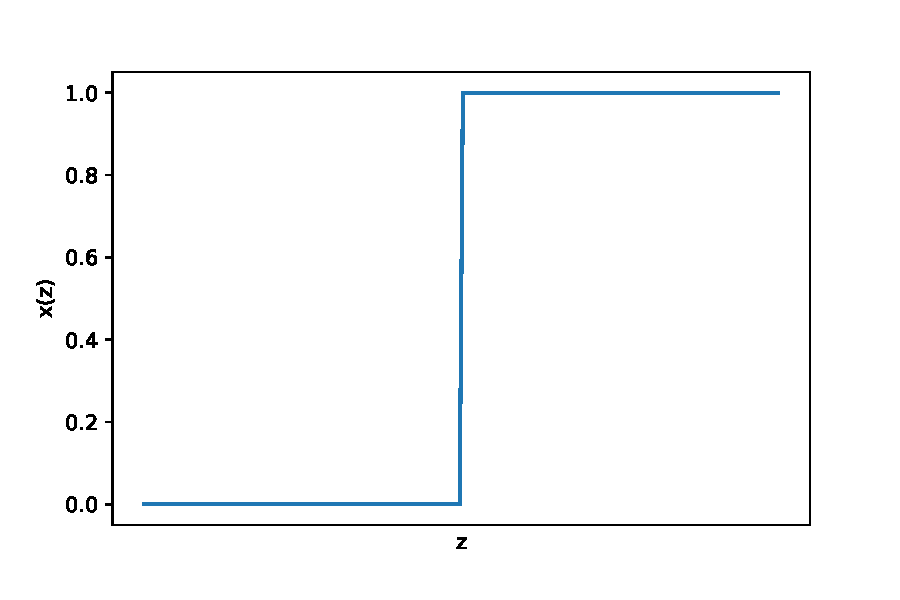
\includegraphics[width=350pt]{pic/jieyuefenpei.pdf}
    \caption{临界标的的示意}
    \label{criticalbid}
\end{figure}

\subsubsection{社会福利最大化带来的问题}
前文中提及的理想机制主要满足DSIC、社会福利最大化、计算有效性特性。然而在背包拍卖中难以完全实现。因为背包问题属于NP-hard问题,难以在多项式时间内准确求解,除非$P=NP$。所以社会福利最大化特性和计算有效性不可兼得。为了解决两者的冲突性,放松DSIC的限制并不能带来任何帮助。若放松社会福利最大化的限制,保证计算有效性,可以通过近似算法在多项式时间内求解社会福利最大问题,但这可能使分配规则单调性被破坏。若放松计算有效性的限制,可以通过动态规划算法在伪多项式时间内对该问题求解。这在问题规模较小或者有较大的算力的条件下是极好的,因为社会福利最大化被精确求解,对应的分配规则一定是单调的,可以被扩展为DSIC机制。

\subsubsection{启发式算法}
利用现有的近似算法,可以得到一个背包拍卖的启发式算法,该算法可以在真实投标的情况下,达到最优社会福利的至少50\%。

\begin{algorithm}[H]
\caption{基于贪心思想的背包问题启发式算法}
对买方根据各自$\frac{b_i}{w_i}$指标进行降序排列,使得$\frac{b_1}{w_1}\geq\frac{b_2}{w_2}\geq \cdots \geq \frac{b_n}{w_n}$\;
以上述序列依次选择胜出者,直到背包无法继续装下,得到胜出者集合$Winners$\;
比较最高标的的买方作为唯一胜出者的社会福利与集合$Winners$的社会福利,返回较大的那个作为最终的胜出者。\;
\end{algorithm}

\subsubsection{算法机制设计}
算法机制设计是算法博弈论中研究较为广泛的一个分支。背包拍卖也是该领域的研究对象之一。算法机制设计的主要模式是尽可能少地放松理想机制中的社会福利最大化限制条件,同时满足DSIC和计算有效性的限制。于单变量环境而言,麦尔森引理将此任务归约至对于具有多项式时间和单调性的分配规则的设计,同时减少社会福利的损失。

算法机制设计与近似算法领域的诸多相似性可能也是其在过去十几年取得较多进展的原因之一。近似算法的主要研究目标是为NP-hard问题设计一种尽可能最优的多项式时间算法。算法机制设计往往也有类似的目标,唯一不同之处是额外需要一个单调性的限制条件。那么,算法机制的设计就被限制于一个可计算模型的设计了。

显示定理可以进一步扩大DSIC机制的有效应用范围。
\begin{theorem}[DSIC机制的显示定理]
对于任意机制$M$,若每个参与者总是有一个占优策略,那么一定存在一个与$M$等价的直接显示DSIC机制$M'$
\end{theorem}

上述定理中的等价意味着,对任意参与者估值向量$\mathbf{v}$,直接显示机制$M'$的结果(价格和分配)与参与者执行占有策略下的机制$M$的结果是一致的。这也说明若要设计具有占有策略的机制,只需要考虑DSIC机制。

\begin{figure}[h]
    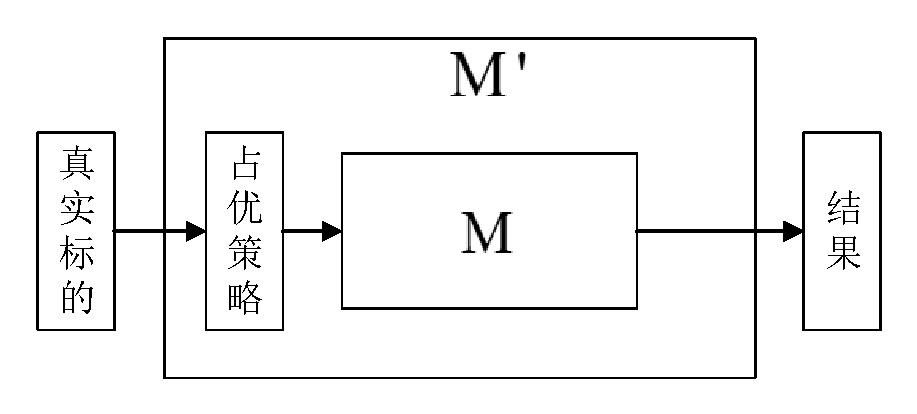
\includegraphics[width=350pt]{pic/revelation.pdf}
    \caption{DSIC机制显示定理的示意}
    \label{revelation}
\end{figure}
如图\ref{revelation}所示,对于任意一个具有占有策略的机制$M$,都可以构建一个以真实估值作为标的输入然后执行各个参与者的占优策略,并最终得到与机制$M$完全一致结果的直接显示DSIC机制$M'$。

若考虑放松DSIC的特性,会损失掉机制的强激励属性。例如在参与者不具有占优策略的机制中,机制设计者需要设定更强的对参与者策略及行为的假设,然后以此判断机制的结果。例如,可以考虑在已知各个参与者私密估值的先验分布的情况下,分析具有贝叶斯纳什均衡的机制。在一些特殊场景需求下,非DSIC机制或许能够取得一些额外的性质。而在较一般的场景中,DSIC的激励特性是极有价值的。

\subsection{税收最大化拍卖}
在前面的机制设计中,社会福利最大化需要求解的目标函数,可以准确求解或者近似求解。卖方的收益在这样的机制中是没有着重考虑的。但是在实际应用中,卖方希望尽可能最大化自身收益是一个极为合理的场景需求。
\subsubsection{贝叶斯分析}
为了比较不同拍卖机制,我们需要一个模型来衡量这些机制在不同的真实估值向量下的税收和。经典的方法是采用贝叶斯分析。考虑这样一个模型:
\begin{itemize}
    \item 单变量环境,且对任意$i$及任意可行解$(x_1,x_2...,x_n)\in X$存在一个常数$M$,使得$x_i\leq M$。
    \item 独立的分布$F_1...F_n$,以及对应的连续概率密度函数$f_1..f_n$。假设参与者$i$的私有估值$v_i$来自于分布$F_i$,且分布$F_i$存在有限一阶矩。
\end{itemize}
另外,机制设计值知道分布$F_1,F_2,F_3,...,F_n$,而参与者不知道。
\begin{definition}[期望税收]
对于一个DSIC机制$(x,p)$,其期望税收为
   \begin{equation}
    \mathbf{E}_{\mathbf{v}\sim\mathbf{F}}{\left[\sum_{i}^{n}{p_i(\mathbf{v})}\right]}
    \end{equation}
\end{definition}
其中$F=F_1\times...\times F_n$。直观来看,直接最大化上式是相对困难的。因而给出虚拟估值的定义。
\subsubsection{虚拟社会福利}
\begin{definition}[虚拟估值]
    对于参与者$i$,其估值及其对应分布分别是$v_i$,$F_i$,则其虚拟估值定义为:
    \begin{equation}
     \varphi_i(v_i) = v_i - \frac{1-F_i(v_i)}{f_i(v_i)}   
    \end{equation}
\end{definition}
由上述定义可知,参与者的虚拟估值仅依赖于他的真实估值与其对应概率分布,而不依赖于其他参与者的信息。然后给出一个引理,该引理是最优拍卖理论的基石。
\begin{lemma}
\label{virtualval}
    对于任意单变量环境、任意概率分布$F_1,F_2...,F_n$、任意DSIC机制$(\mathbf{x},\mathbf{p})$、任意参与者$i$、任意其他参与者的估值$\mathbf{v_{-i}}$,
    \begin{equation}
       \mathbf{E}_{v_i\sim F_i}[p_i(\mathbf{v})]= \mathbf{E}_{v_i\sim F_i}[\varphi_i(v)\cdot x_i(\mathbf{v})]
    \end{equation}
\end{lemma}
上述引理的含义为:任意参与者支付$p_i$的期望等于该参与者所获得的虚拟价值$\varphi_i(v)\cdot x_i(\mathbf{v})$的期望。

基于引理\ref{virtualval},可得如下重要定理。
\begin{theorem}[期望税收等于期望虚拟社会福利]
    对于任意单变量环境、任意估值的概率分布$F_1,...,F_n$,任意DSIC机制$(\mathbf{x},\mathbf{p})$,
    \begin{equation}
    \label{expvirtualwelfare}
    \mathbf{E}_{\mathbf{v}\sim\mathbf{F}}{\left[\sum_{i}^{n}{p_i(\mathbf{v})}\right]}=\mathbf{E}_{\mathbf{v}\sim\mathbf{F}}{\left[\sum_{i}^{n}{\varphi _i(v_i)*x_i(\mathbf{v})}\right]}
    \end{equation}
\end{theorem}

上述定理的重要意义在于,其在相同的分配规则可行集内,将难以直接最大化的期望税收转化依赖于分配函数的最大化期望虚拟社会福利。在式\ref{expvirtualwelfare}中,着重考虑等式右边的部分$\mathbf{E}_{\mathbf{v}\sim\mathbf{F}}{\left[\sum_{i}^{n}{\varphi _i(v_i)*x_i(\mathbf{v})}\right]}$。对于概率分布$\mathbf{F}$及虚拟估值$\varphi_i(v_i)$,机制设计者是无法控制或者改变的。只有分配规则$\mathbf{x(v)}$由机制设计者制定。为了最大化期望虚拟社会福利,可以对前式取关于$\mathbf{v}$的条件期望,得到
\begin{equation}
\mathbf{E}_{\mathbf{v}\sim\mathbf{F}}{\left[\mathbf{E}\left[\left.\sum_{i}^{n}{\varphi _i(v_i)*x_i(\mathbf{v})}\right|\mathbf{v}\right]\right]}
\end{equation}
原问题则转化为对相应条件期望的最大化,由上式可知,这等价于选择使虚拟社会福利$\sum_{i}^{n}{\varphi _i(v_i)*x_i(\mathbf{v})}$最大化对应的分配规则。

值得注意的是,上述分配规则必须满足单调性,否则前述定理的前提条件$(\mathbf{x},\mathbf{p})$是DSIC机制无法被满足。为了说明虚拟社会福利对应分配规则的单调性,有如下定义。
\begin{definition}[正规分布]
若虚拟估值函数$v-\frac{1-F(v)}{f(v)}$是非单减的函数,则概率分布$F$称为正规分布。 
\end{definition}
进一步可知,若所有参与者的估值分布$F_1,F_2,...,F_n$均是正规分布,则虚拟社会福利最大化对应的分配规则一定是单调的。从而上述税收最大化的设计可以完成其闭环流程,如下所示:

\begin{algorithm}[H]
\caption{期望税收最大化}
假设:每个参与者估值的分布$F_i$均为正规分布\;

将每个参与者的真实估值$v_i$转化为虚拟估值$\varphi_i(v_i)$\;
在可行集中选择可行解$\mathbf{x}$使得虚拟社会福利最大化$\sum_{i}^{n}{\varphi _i(v_i)*x_i(\mathbf{v})}$\;
根据麦尔森引理计算支付向量$\mathbf{p}$\;
\end{algorithm}

上述流程为单变量环境下,期望税收最大化即最优拍卖的一般设计流程。
\subsection{多变量环境}
前面的理论以单变量环境为基础,参与者的隐藏信息为单个值。而更一般的是多变量环境,即参与者的隐藏信息为多个值。在一般的多变量机制中有:

\begin{enumerate}
    \item $n$个策略性的参与者
    \item 有限的结果集合$\Omega$
    \item 每个参与者$i$具有私密的非负估值函数$v_i(\omega),\omega \in \Omega$。
\end{enumerate}

此时的社会福利被定义为$\sum_{i=1}^{n}{v_i(\omega)}$。在多变量环境中有重要的结论:
\begin{theorem}
    任意多变量环境都存在一个社会福利最大化的DSIC机制。
\end{theorem}
该DSIC机制被称为VCG机制,其分配规则和支付规则分别为:
\begin{equation}
 \mathbf{x}(\mathbf{b})=argmax_{\omega \in \Omega}\sum_{i=1}^{n}{b_i(\omega)}
\end{equation}
\begin{equation}
p_i(\mathbf{b})=\left(\max_{\omega\in\Omega}\sum_{j\neq i}{b_j(\omega)}\right)-\sum_{j\neq i}b_j(\omega^\star)    
\end{equation}
其中,$\omega^\star$是上述分配规则选出的结果。在多变量环境下,由于VCG机制的存在,似乎优秀激励性质的机制设计变得可行。然而事实并非如此。一方面,其最大化社会福利问题基本都是NP-hard问题,难以有效实现。每个参与者标的的长度随问题规模呈指数级增长,存储、传输这些多维的标的也将带来极大的时空花费。另一方面,VCG机制仅能保证社会福利最大,而在税收等其他方面并不具有更多的优秀性质。
\section{动态规划}
动态规划,是一种在数学、计算机科学、经济学等领域中使用的解决复杂问题的方法。它把原问题分解为相对简单的子问题来进行求解。动态规划常常适用于具有重叠子问题和最优子结构性质的问题,而其所需时间基本原少于朴素算法。

动态规划适用的情况:

\begin{description}
    \item[最优子结构]若问题的最优解所包含的子问题的解也是最优的,那么该问题就具有最优子结构。
    \item[无后效性]子问题的解一旦确定就不再改变。问题的求解呈现明显的阶段性,当前阶段的最优解不依赖与后续阶段决策。
    \item[子问题重叠]原始问题划分的子问题中有相互重叠的部分,这些重叠的子问题只被计算一次,可以将指数时间级的枚举算法转化为伪多项式时间的求解,极大提升算法时间效率。
\end{description}

\subsection{背包问题}
背包问题是一种组合优化的NP完全问题,问题可以描述为:给定一组物品,每种物品都有自己的重量和价格,在限定的总重量内,我们如何选择,才能使得物品的总价格最高。相似的问题常出现在组合数学,计算复杂性理论,密码学和应用数学等领域。
\subsubsection{定义}
问题中有n种物品,物品j的重量为$w_i$,价格为$p_i$。假定所有物品的重量和价格都是非负的,背包能承受的最大重量为$W$。

若每种物品只能选择0个或者1个,则为0-1背包问题。
\begin{align}
    \max_{\vec{x}} \quad&\sum_{i=1}^{n}{p_ix_i}\\
    s.t                     
                            \quad& \sum_{i=1}^{n}{w_ix_i} \leq W,\quad x_i\in\{0,1\}\notag 
\end{align}
若每种物品都有个数限制,最多取$b_i$个,则为有界背包问题。
\begin{align}
    \max_{\vec{x}} \quad&\sum_{i=1}^{n}{p_ix_i}\\
    s.t                     
                            \quad& \sum_{i=1}^{n}{w_ix_i} \leq W,\quad x_i\in\{0,1,...,b_i\}\notag 
\end{align}
若每种物品数量不受任何限制,则为无界背包问题。
\begin{align}
    \max_{\vec{x}} \quad&\sum_{i=1}^{n}{p_ix_i}\\
    s.t                     
                            \quad& \sum_{i=1}^{n}{w_ix_i} \leq W,\quad 0\leq x_i\notag 
\end{align}

上述背包问题的精确求解都可以通过动态规划在伪多项式时间内解决。以此为基础还能构建FPTAS的近似算法。
\subsubsection{泛化物品}
考虑这样一种物品,它并没有固定的费用和价值,它的价值随着分配给它的费用变化而变化。更严格的定义是,在背包容量为$V$的背包问题中,泛化物品是一个定义域为$\{0,1,2,...,W\}$的函数$h$,当分配给它的费用为$v$时,能够得到的价值就是$h(v)$。

若给定了两个泛化物品$h$和$l$,需要一定的费用从这两个泛化物品中得到最大的价值。可以通过枚举费用在两个泛化物品之间的分配即可。类似的,可以求得新的泛化物品对应的函数$f$。即
\begin{equation}
    f(w)=max\{h(k)+l(w-k)|0\leq k \leq w\}
\end{equation}

由上式可知,$f$是一个由$h$和$l$得出的新的泛化物品,该过程也可称为泛化物品$h$与泛化物品$l$的求和,每次求和的时间复杂度为$O(W^2)$。泛化物品的概念可以应用于背包问题的一系列拓展及变体中。

\section{本章小结}
本章首先介绍了机制设计、麦尔森引理、最优拍卖、背包拍卖等算法机制设计中的关键概念。然后简要说明了动态规划的思想及背包问题的中泛化物品的概念。为后文针对具体场景进行机制设计及分析做准备。

\chapter{简单可并行计算下的机制}
\section{多方数据价值共享计算模式}
现有的大数据的应用模式与数据隐私安全问题存在不可调和的矛盾。一方面,大数据创造的价值依赖于数据整合并较好地应用相关数据挖掘算法。而整合意味着开放,开放必然引入安全隐患。因而,此节简要介绍一种多方数据价值共享计算\footnote{在后文的分析中可能简称为多方计算}的模式。该模式并不直接整合数据,而是对计算任务进行分解拆分,使之能够在各数据中心\footnote{本文以数据中心作为数据拥有者的代表}本地完成相应的分布式计算,并将计算结果传输给控制节点。这些计算结果不会引入原始数据的隐私安全风险。然后由控制节点实现结果的整合。对于复杂的计算问题,该过程可能包含若干次迭代操作。
\begin{figure}[h]
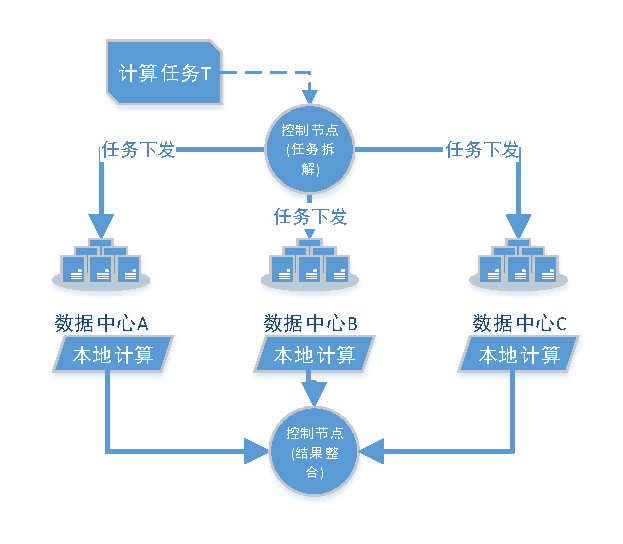
\includegraphics[width=350pt]{pic/yuanweishiyi.pdf}
\caption{多方数据价值共享计算示意}
\label{yuanweishiyi}
\end{figure}

值得注意的是,该计算模式中,各个数据中心的计算任务仅依赖于本地数据,即数据本身分布于各地且在整个计算过程中不通过网络传输或者转移。这可以有力保证数据的隐私安全性。如何将计算任务T根据现有数据分布进行子任务切分是控制节点的问题,本文并不对此进行说明,只是假设控制节点可以有效地完成此任务。

对于各个数据拥有者(例如图\ref{yuanweishiyi}中的数据中心)来说,参与到多方价值计算模式必然给自身带来损失。系统的设计者需要给予经济奖励,来激励更多的数据价值共享。而随着参与者的增多,提供相同计算内容的参与者之间的竞争增加,如何选择胜出者是一个重要问题,因而需要设计合理的价格体系来保证系统的有效运行。
\begin{figure}[h]
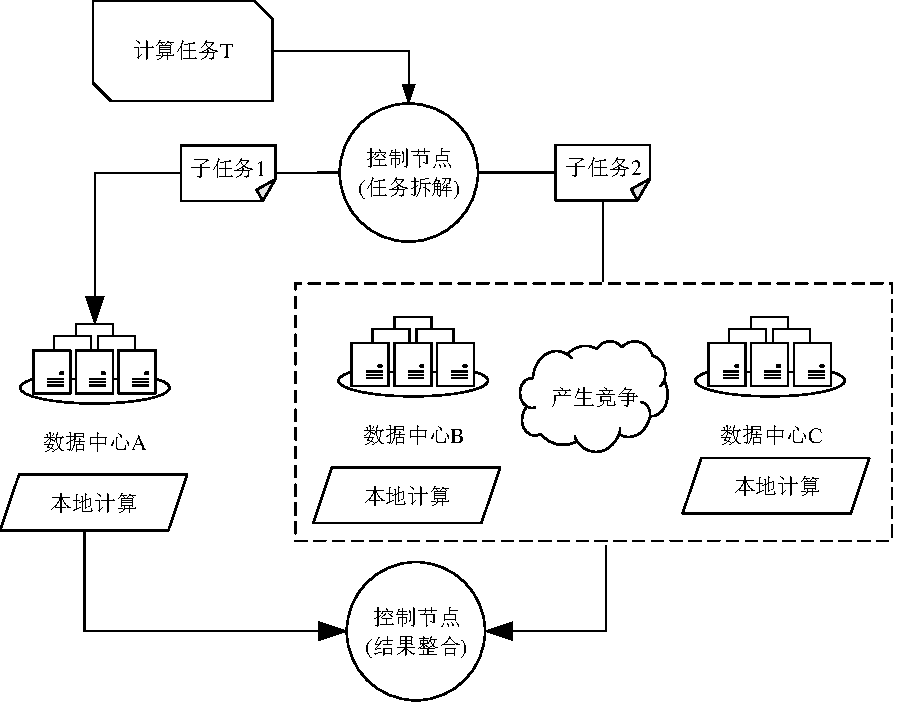
\includegraphics[width=350pt]{pic/yuanweijili.pdf}
\caption{多方数据价值共享中的竞争}
\label{yuanweijili}
\end{figure}
如图\ref{yuanweijili}所示,数据中心B和数据中心C都可以在依赖于本地数据的情况下提供对子任务2的计算,此时两者产生竞争,如何确定最终执行子任务2的数据中心是一个较为重要的问题。而本章的后续内容及第四章的内容主要是针对该计算模式,在不同场景下进行相应的机制设计。

\section{简单可并行计算基础拍卖模型}

\subsection{问题描述}
在简单可并行计算的场景中,上述多方计算任务T可以被控制节点根据现有的数据分布情况划分为一定数量的子计算任务。这些依赖于本地数据的子计算任务可以在各个数据中心完全并行的完成,然后由控制节点对计算结果进行一次整合得到原任务的解。而这些子计算任务大多是同构的(例如,对图片数据进行特征提取)。每个子计算任务称为一个单位(unit)的多方计算。

\subsection{形式化定义}
\label{jichumoxingdingyi}
首先给出相关合理假设:
\begin{itemize}
    \item 假设1:参与者是有限理性的个体,总是执行理性条件下最大化各自效用函数的策略,且不存在共谋。
    \item 假设2:除参与者对多方计算任务代价的内心估值为私密知识以外,其余均为公共知识,为平台方和其它参与者所知。
\end{itemize}

机制中以虚拟代币作为货币。机制中有$n$个参与者$\mathbf{agent}$可以进入多方计算任务$T$的竞拍环节。多方计算任务$T$共需要$datademand$单位的计算。对于$1\leq i\leq n$,参与者$agent_i$可以针对任务书$T$提供$datacount_i$单位的多方计算任务。
而参与者$agent_i$拥有私密值$0 \leq val_i = INCENT-cost_i$,$INCENT$是平台方给予胜出者的每单位计算任务的固定奖赏,由平台方或者多方计算任务发起者确定\footnote{本文中不特意区分平台方与计算任务发起者,因为他们可能是同一角色}。$0 \leq cost_i \leq INCENT$,否则,参与者$agent_i$应当退出此次竞拍来避免自己受损。 于是,$val_i$表示$agent_i$对购买每单位多方计算任务带来的真实价值。其$val_i$只对参与者$agent_i$可见,平台方及其余参与者不可见。在机制中,每个参与者会提交自己的标的$b_i$,形成标的向量$\mathbf{bid}$。分配函数$\mathbf{allocation}(\mathbf{bid})$也是一个向量,表示了机制对参与者分配的多方计算任务数量。$agent_i$的效用函数定义为准线性函数$utility_i = val_i*allocation_i-payment_i$。总社会福利$\mathbf{SW}$定义为$\sum_{i=1}^n{val_i*allocation_i}$,其是所有参与者的效用函数与平台方收益的总和。即:$\mathbf{SW} = \sum_{i=1}^n{utility_i}+\sum_{i=1}^{n}{payment_i}$

\subsection{分析及求解}
本文的目标是设计一种参与者具有占优策略的拍卖机制。由显示定理可知,对于任意一个参与者总是具有占优策略的机制$M$,总是存在一个等价的直接显示(direct-revelation)占优策略激励相容(DSIC)机制$M'$。因此,本文在DSIC机制的范围中寻找合适的解。而在前述基础拍卖模型定义中,参与者的私密值仅为其对购买多方计算任务的收益真实估值$val_i$,且效用函数为准线性函数。这属于单变量环境,需要麦尔森引理来主导机制设计的流程。

假设所有参与者已经真实地表达多方计算任务的估值,并给出标的,即$\mathbf{bid} = \mathbf{val}$。 此时对于平台方来说,社会福利最大化等价于最优化问题\ref{jichumoxing}。

\begin{align}
    \label{jichumoxing}\max_{\vec{allocation}} \quad&\sum_{i=1}^{n}{bid_i*allocation_i}\\
    s.t                     \quad& 0\leq allocation_i\leq datacount_i,\quad allocation_i = {0,1,2...}\notag\\
                            \quad& \sum_{i=1}^{n}{allocation_i} = datademand\notag 
\end{align}

给出贪心算法:\footnote{本文中数组下标均从1开始计数}
\footnote{可以通过first和second来分别指代二元组的第一、二关键字}时间复杂度$O(n)$

\begin{algorithm}[H] 
    \KwIn{$\mathbf{datacount},\mathbf{bid},datademand$}
    \KwOut{$\mathbf{allocation}$}
    $i \leftarrow 1$\;
    $total \leftarrow datademand $\;
    对二元组序列$list = \{(bid_j,j)|1 \leq j \leq n\}$以第一关键字进行降序排列,第一关键字相同的情况下,以第二关键字升序排列\;
    \While{total > 0}{
        \If{i > n}{
            datademand单位的计算任务无法被分配完毕,返回错误信息。
            break\;
        }
        $temp \leftarrow \min(total,\quad datacount_{list[i].second})$\;
        $total \leftarrow total - temp$\;
        $allocation_i \leftarrow temp$\;
        $i \leftarrow i + 1$\;
    }
\caption{贪心算法求解基础拍卖模型}
\label{tanxin}
\end{algorithm}

\begin{theorem}
算法\ref{tanxin}是问题\ref{jichumoxing}的解。
\end{theorem}

\begin{proof}
    算法\ref{tanxin}的思想是在供应$datademand$有限的情况下,优先满足代价估值$bid_i$更大的参与者的需求。假设存在一个更优解$S^1(SW^1 > SW)$与该思想相悖。即存在$1 \leq i \neq j \leq n,bid_i > bid_j$, 使得$allocation_i < datacount_i \text{, } allocation_j > 0$。不妨将分配给参与者$agent_j$的$temp = min(datacount_i - allocation_i,allocation_j)$单位计算任务重新分配给参与者$agent_i$,得到解$S^2$,此时新的社会福利$SW^2= SW^1- temp*bid_j + temp*bid_i=SW^1+temp*(bid_i-bid_j)$,由前述条件可知,$temp > 0$且$bid_i - bid_j > 0$。易得,$SW^1<SW^2 $。继续对$S^2$执行以上流程,直到前提条件不满足。此时,解$S^n$优先满足代价估值更大的参与者的需求。由贪心算法可知$SW^n = SW$,则$SW^1<SW^2...<SW^n=SW$,这与假设不符。故不存在上述更优解。
\end{proof}

分配函数已经确定,为了应用麦尔森引理确定价格函数,需要首先分析分配函数关于标的$bid_i$的单调性。

\begin{theorem}
    对于任意参与者$agent_i$以及任意$\mathbf{bid_{-i}}$\footnote{表示除$bid_i$分量以外的总标的向量},算法\ref{tanxin}所示分配规则$allocation_i(z,\mathbf{bid_{-i}})$是关于$agent_i$的标的$z$的单调不减函数。
\end{theorem}

\begin{proof}
   在保持其余标的不变的情况条件下,若$agent_i$的标的$z$变大,则其在算法\ref{tanxin}中list序列中的排位只会更加靠前,从而获得更高优先级的分配权力。而算法的不确定性已经由第二关键字排序消除。
\end{proof}



\begin{figure}[h]
    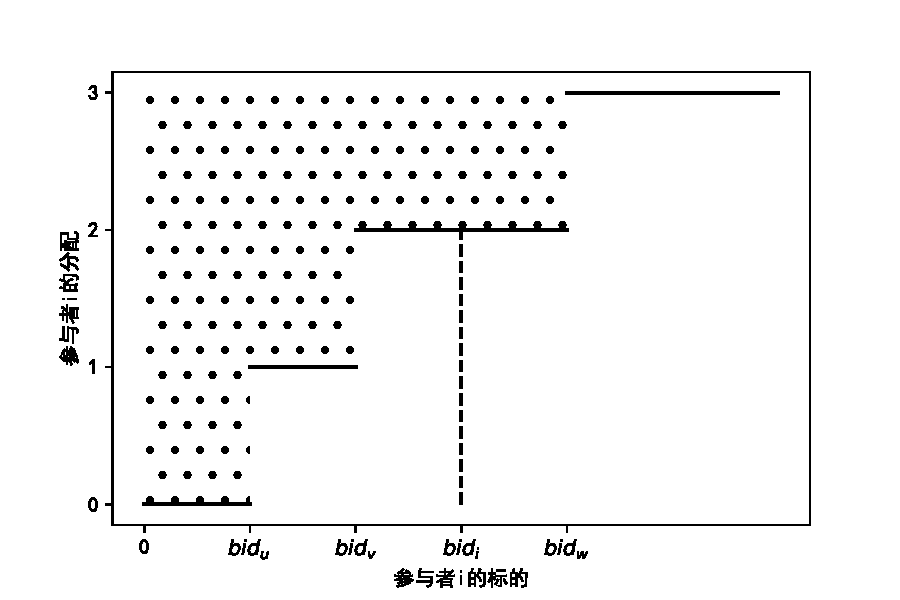
\includegraphics[width=350pt]{pic/tanxin_allocation.pdf}
    \caption{贪心算法分配函数示例}
    \label{tanxin_allocation}
\end{figure}

不失一般性,$allocation_i(z,\mathbf{bid_{-i}})$函数图像如图\ref{tanxin_allocation}所示。
根据麦尔森引理,阴影部分面积即为$agent_i$向平台方支付的报酬。由图像可知,需要求解出这些阶跃变化值。根据贪心算法的流程,假设已知根据$\mathbf{bid}$降序排列的$\mathbf{datacount}$前缀和数组$\mathbf{prefix}$,则可以迭代求出这些阶跃值,从而求得阴影部分总面积。其余$agent$的代价计算亦然。总体$\mathbf{payment}$计算具体细节如算法\ref{tanxin_zhifu}所示,算法时间复杂度$O(n^2)$。

\begin{algorithm}[H]
    \KwIn{$\mathbf{datacount},\mathbf{bid},datademand$}
    \KwOut{$\mathbf{payment}$}
    运行算法\ref{tanxin},获得list\;
    \tcp{根据标的排序求count的各前缀和}
    prefix 置为初始值为0的数组\;
    \For{$i = 1$ \KwTo $n$}
    {
        \If{i > 1}{
            $prefix[i] \leftarrow prefix[i-1]$\;
        }
        $prefix[i]  += datacount_{list[i].second}$\;
    }
    \tcp{求每个参与者的支付$payment_i$}
    \For{$i = 1$ \KwTo $n$}
    {
        $payment_{list[i].second} \leftarrow 0$\;
        \tcp{ind存储遍历下标}
        $ind \leftarrow i + 1$
        \tcp{y存储当前分配值}
        \eIf{$i = 1$}
        {
            $y \leftarrow min(datademand,datacount_{list[i].second})$\;
        }{
        $y \leftarrow min(max(datademand - prefix[i-1],0),datacount_{list[i].second})$\;
        }
        \While{$ind \leq n$ 且 $y > 0$}
        {
            $newy \leftarrow min(max(datademand - prefix[ind]+ datacount_{list[i].second},0),datacount_{list[i].second})$\;
            $payment_{list[i].second} += (y - newy)*list[ind].first$\;
            $y \leftarrow newy$\;
            $ind += 1$\;
        }
    }
\caption{贪心算法求解基础拍卖模型的支付流程}
\label{tanxin_zhifu}
\end{algorithm}

\section{多重指标限制}
\label{dptou}
\subsection{问题描述}
    多方计算任务竞拍场景中,平台方或者任务提交方对于任务购买方存在总体偏好设置或者限制条件。例如:平台方可以出于总体计算结果来源异构性等需求要求竞拍胜出者的数量不能超过某给定阈值;或者要求多方计算任务$T$的总体响应时间不能大于给定目标值。在本场景中,参与者会被赋予不同的信誉等级及可靠性评估。而平台方也可以根据自己对任务难易程度的估量,制定不同的限制条件。假设限制指标集$Limit$是有限集。本文中使用表\ref{zhibiao}所示指标作为分析。

\newcommand{\tabincell}[2]{\begin{tabular}{@{}#1@{}}#2\end{tabular}} %放在导言区

\begin{table}[h]
\caption{限制指标集}
\label{zhibiao}
\begin{tabular}{cp{10em}cc}
    \toprule
    指标名称& 描述&符号&产生方式\\
    \midrule
    一级参与者的数量阈值&来自信誉系统\footnote{本文并不给出信誉系统的计算方式,这可以由系统设计者自定义}&$Parti_1$&由平台方或任务方确定\\
    二级参与者的数量阈值& 同上&$Parti_2$&由平台方或任务方确定\\
    三级参与者的数量阈值& 同上&$Parti_3$&由平台方或任务方确定\\
    总体响应时间和&各个胜出者完成来自任务$T$所指派计算花费的时间总和&TIME&由平台方或任务方确定\\
    计算需求量&&datademand&任务$T$固有属性\\
    \bottomrule
\end{tabular}
\end{table}

上述指标集中,前三项来自于对参与者的信誉等级及可靠性评估。前三项指标是同类指标,以第一项为例,它意味着平台方要求任务$T$的胜出者中一级参与者刚好有$Parti_1$个。第四项指标衡量了多方计算任务$T$的总体完成效率。$TIME$值越小,意味平台方对于任务的响应要求越高,对于拍卖环节的限制也就更强。第五项$datademand$是来自于多方计算任务本身的需求,机制需要尽可能使$datademand$被满足,这里也将其视为平台方对多方计算任务分配的限制指标之一。
\subsection{形式化定义}
\label{dpdingyi}
在\ref{jichumoxingdingyi}节所示基础上引入上述指标集限制条件。$level_i\in {1,2,3}$为$agent_i$的信誉及可靠性评估。对于$1\leq j \leq 3$,胜出者集合中第$j$级参与者数量$=parti_j$。$timeperunit_i$是$agent_i$关于$任务T$完成每单位
计算任务所花费的时间。$transmitcost_i$是$agent_i$向平台方提交结果数据所花费的平均时间,主要由网络时延、吞吐量等因素决定。分配规则需要满足时效性要求指标:$\sum_{i=1}^{n}{timeperunit_i*allocation_i+\mathbf{I}(allocation_i > 0)*transmitcost_i} < TIME$
\footnote{$\mathbf{I}(\text{表达式}) = \begin{cases}{}
        0&,\text{表达式为假}\\
        1&,\text{表达式为真}
        \end{cases}$
}%,$timeperunit_i$和$transmitcost_i$的定义见\ref{dpdingyi}节。}
社会福利$SW$的定义仍然不变。
假设所有参与者已经真实地表达多方计算任务的估值,并给出标的,即$\mathbf{bid} = \mathbf{val}$,此时对于平台方来说,社会福利最大化等价于最优化问题\ref{dpmoxing}
\begin{align}
    \label{dpmoxing}\max_{\vec{allocation}} \quad&\sum_{i=1}^{n}{bid_i*allocation_i}\\
    s.t\quad& 0\leq allocation_i\leq datacount_i,\quad allocation_i = {0,1,2...}\notag\\
        \quad& \sum_{i=1}^{n}{allocation_i} = datademand\notag\\
        \quad& \left(\sum_{i=1}^{n}{timeperunit_i*allocation_i+\mathbf{I}(allocation_i > 0)*transmitcost_i}\right) < TIME\notag\\
        \quad& \left(\sum_{i=1}^{n}{\mathbf{I}(allocation_i > 0,level_i = j)}\right)=parti_j, j = {1,2,3}\notag
\end{align}

\subsection{分析及求解}
最优化问题\ref{dpmoxing}是一个NP-hard问题,此处尝试以动态规划的方式进行求解。拟定6维状态$dp[i,j,a,b,c,t]$,表示考虑前$i$个参与者,刚好分配$j$单位多方计算任务,其中一级参与者$a$个,二级参与者$b$个,三级参与者$c$个,最多花费$t$单位总时间,所能够获得的最大收益。通过枚举分配给$agent_i$的计算任务数量,可以得到状态转移方程\ref{dpfangcheng}。

\begin{gather}
\label{dpfangcheng}  
dp[i,j,a,b,c,t] = max
\begin{cases}
1 \leq k \leq datacount_i \\
\text{If} \quad level_i = 1,\\
dp[i-1,j-k,a-1,b,c,t-k*timeperunit_i-transmitcost_i]+ k*bid_i,\\
\text{If}\quad level_i = 2,\\
dp[i-1,j-k,a,b-1,c,t-k*timeperunit_i-transmitcost_i]+ k*bid_i,\\
\text{If} \quad level_i = 3,\\
dp[i-1,j-k,a,b,c-1,t-k*timeperunit_i-transmitcost_i]+ k*bid_i,\\
\text{all condition},\\
dp[i-1,j,a,b,c,t]
\end{cases}\\
dp[0,0...datademand,0...parti_1,0...parti_2,0...parti_3,0...TIME] =-\infty \notag\\
dp[0,0,0,0,0,0...TIME] = 0 \notag
\end{gather}
上述转移方程中,值得一提的是状态的初始化方法。考虑最优化问题\ref{dpmoxing}的限制条件可知,只有总体响应时间和是不等式限制,其余四项限制指标均等式。这可以通过设置初始状态的合法性来解决。如\ref{dpfangcheng}所示,在限制指标张成的五维空间中,仅有关于运行时间的一维子空间\footnote{此处并非完整定义的子空间}被赋予合法性。其余非法状态置$-\infty$。当限制指标集扩展时,针对不同类型的限制属性也可以按此思路进行初始状态设定。
为了减少状态存储,转移方程\ref{dpfangcheng}可以记忆化搜索的方式进行。
\begin{algorithm}[H]
    \KwIn{$\mathbf{datacount,timeperunit,level,bid},datademand$,及\ref{dpdingyi}节中定义的限制指标}
    \KwOut{$\mathbf{allocation}$}
    对参与者按照默认优先级进行排序,优先级较高的排位靠前。
    $Search(n,datademand,parti_1,parti_2,parti_3,TIME)$\;
    以最优路径对$\mathbf{allocation}$进行赋值\;
    \;
    $Search(i,j,a,b,c,t)$定义为:\;
    检查状态是否访问过,是则直接返回最优解,否则继续向下。\;
    根据方程\ref{dpfangcheng}所示进行状态转移\;
    \For{$i \leftarrow 0$ \KwTo $k$}{
        Search(新的状态)
    }
    记录当前状态最优值,若存在多个最优解,选择$k$值较小的那个,同时记录最优路径。\;
\caption{记忆化搜索}
\label{jiyihua}
\end{algorithm}

\begin{theorem}
对于任意参与者$agent_i$以及任意$\mathbf{bid_{-i}}$,算法\ref{jiyihua}所示分配规则$allocation_i(z,\mathbf{bid_{-i}})$是关于$agent_i$的标的$z$的单调不减函数。
\end{theorem}
\begin{proof}
\label{dpdandiao}
将$agent_i$移至所有参与者的最后一位。由算法\ref{jiyihua}及转移方程\ref{dpfangcheng}可知,参与者$agent_i$的分配$allocation_i$依赖于子空间$dp[n-1,,,,,]$中$datacount_i+1$个状态(分别对应于分配0、1、2...$datacount_i$件计算任务),以及$bid_i$的值。$dp[i-1,,,,,]$中的状态由参与者的许多信息(包括$\mathbf{bid_{-i}}$)及所有环境参量(如\ref{dpdingyi}节中定义的限制指标)决定。因此其不受$bid_i$影响。当$bid_i$变化时,这些状态可以看做固定值。

记$allocation_i(z,\mathbf{bid_{-i}})$为$al_i(z)$,$dp[i-1,,,,,]$中对应的$datacount_i+1$个状态分别为$ndp[0],ndp[1],...ndp[datacount_i]$。不妨假设$a < b$, 且当$bid_i = a$时,$al_i(z) = j$。这意味着$ndp[j]+j*a$是$\{ndp[k] + k*a|0 \leq k \leq j\}$中的极大值。此时再考虑$bid_i=b$时的情景。对于$ 0\leq k\leq j$,对应的状态分别为$ndp[k]+k*b=ndp[k]+k*a+k*(b-a)$,由于$ndp[k]+k*a\leq ndp[j]+j*a$(来自于$bid_i=a$的假设),且$k*(b-a)\leq j*(b-a)$,所以$ndp[k]+k*b \leq ndp[j]+j*b$。那么$al_i(a)\leq al_i(b)$
\end{proof}

为了确定多重指标限制问题下的价格函数,针对每一个$agent_i$,需要确定证明\ref{dpdandiao}中$dp[n-1,,,,,]$子空间中的$datacount_i+1$个状态的值。然后根据这些值找出分配函数$al_i(z)$中的那些阶跃点。由于本场景中,对于每个阶跃点,其$y$轴的阶跃值仅为1。那么可以根据麦尔森引理,求得$agent_i$所需支付的价格。
\begin{equation}
\label{jieyuedian}
 \begin{aligned}
 ndp[1]+1*b_1&=ndp[0]\\
 ndp[2]+2*b_2&=ndp[1]+b_2\\
 ndp[3]+3*b_3&=ndp[2]+2*b_3\\
 &\vdots\\
 ndp[k]+k*b_k&=ndp[k-1]+(k-1)*b_{k-1}
 \end{aligned}
\end{equation}

解方程组\ref{jieyuedian},可以得到所有阶跃点序列$b_1,b_2,b_3...b_k$。值得注意的是,该序列不一定单调递增。

\setcounter{footnote}{0}

\begin{algorithm}[H]
\KwIn{$\mathbf{datacount,timeperunit,level,bid},datademand$,及\ref{dpdingyi}节中定义的限制指标}
    \KwOut{$\mathbf{payment}$}
    运行算法\ref{jiyihua},得到分配$allocation_i$\;
    \For{每个参与者$agent_i$}
    {
        $payment_i \leftarrow 0$\;
        将$agent_i$移至末位,重新运行算法\ref{jiyihua},得到:\;
        $ndp[0] = dp[n-1,datademand,parti_1,parti_2,parti_3,TIME]$\;
        $ndp[k] = dp[n-1,datademand-k,parti_1-\mathbf{I\footnotemark}(level_i=1),parti_2-\mathbf{I}(level_i=2),parti_3-\mathbf{I}(level_i=3),TIME-k*timeperunit_i-transmitcost_i],1\leq k\leq datacount_i$\;
        $record \leftarrow 0$\;
        \For{$ind \leftarrow 1$\KwTo $allocation_i$}{
            $record \leftarrow max(record,ndp[ind-1] - ndp[ind])$\;
            $payment_i \leftarrow payment_i + record$\;
        }
    }
\caption{多重指标限制问题价格规则}
\label{dp_zhifu}
\end{algorithm}
\footnotetext{$\mathbf{I}(\text{表达式}) = \begin{cases}{}
        0&,\text{表达式为假}\\
        1&,\text{表达式为真}
        \end{cases}$
}

\section{机构场景扩展及额外偏好设置}
\subsection{问题描述}
在本章场景中,多方计算任务$T$竞拍流程中的参与者的真实角色是拥有计算资源及相应数据访问权限的计算节点。这些计算节点隶属于不同的部门机构。就相对严格而紧密的组织而言,其部门机构可能存在较为显著的上下级关系。这种关系最典型的案例是树形关系。如\ref{jigoushu}所示。在这种树形关系中,各机构可能会出于成本管理、机构职能、安全性保障等多方面因素对其自身及下属机构参与多方计算任务提出新的要求及限制。例如,\ref{zhibiao}所示的各种限制性指标。这些要求及限制形成每个机构的偏好信息。如图\ref{jigoushu},每个机构都拥有一个偏好信息描述。(图中并未完全画出所有偏好信息)

\begin{figure}[h]
\center
    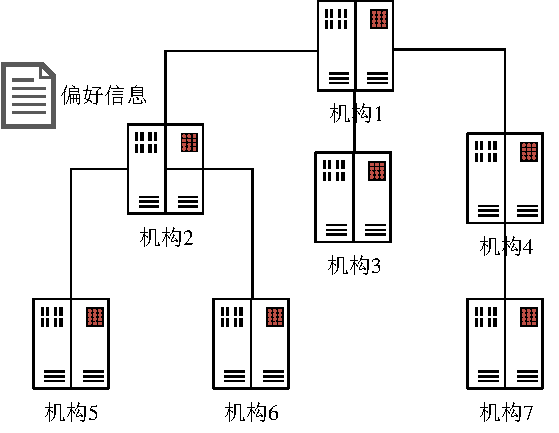
\includegraphics[width=350pt]{jigou_tree.pdf}
    \caption{机构部门间的树形关系}
    \label{jigoushu}
\end{figure}

另一方面,同一机构内部可能具有多个可提供计算能力的单位,他们具有相同的多方计算数据访问权,但他们的计算能力、质量又是参差不齐的。当同一机构内部的不同计算单位作为参与者进入到多方计算任务$T$的竞争环节中时,多个参与者可能提供的是数据相同而计算方式或者服务质量具有差异的多方计算。相同的计算内容对于同一多方计算任务$T$来说是冗余的。因此在前述场景中,这些数据同质的参与者之间实质存在互斥关系。即在这些数据同质的参与者中,分配规则最多只能选择1个胜出者。同一机构可能拥有多个不同的数据源,因此在一家机构内部也可能存在多组这样的互斥关系。目前我们只考虑在来自一家机构的参与者中存在数据同质的现象。
\begin{figure}[h]
    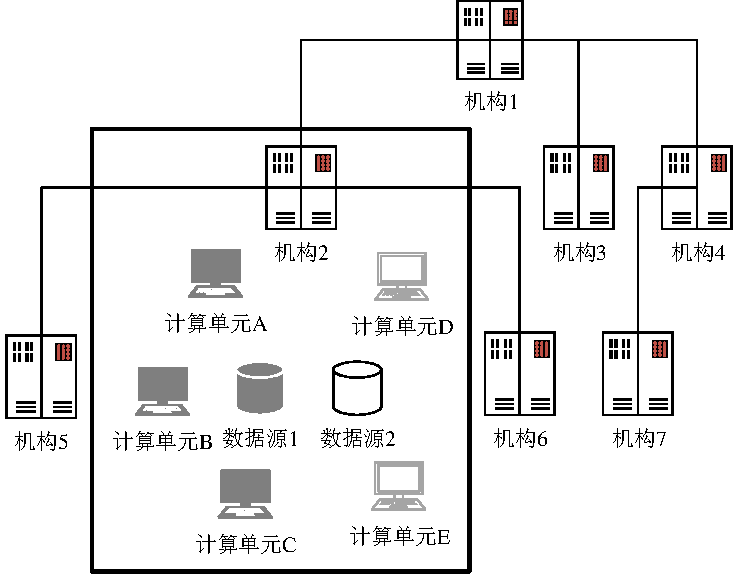
\includegraphics[width=350pt]{huchi_tree.pdf}
    \caption{机构内部参与者的互斥关系示例}
    \label{huchishu}
\end{figure}

在图\ref{huchishu}的示例中,机构2的计算单元$A,B,C$拥有数据源$1$的访问权,计算单元$D,E$拥有数据源$2$的访问权。当这些计算单元参与至多方计算任务竞争环节时,计算单元$A,B,C$及$D,E$中各自最多只能有一个胜出者。
\subsection{形式化定义}

在前文的形式化定义中增加机构的概念。机制中共有$m$个机构,所有参与者$agent_i,1 \leq i \leq n$隶属于这些机构。每个机构具有参与者偏好$prefer_i$,描述了其对自身管辖的部门参与多方计算的限制条件。现仅考虑如下限制:该机构及其管辖部门的参与者所提供的总多方计算任务不能超过$limit_i$单位。此节的分析及结论可以被推广至所有限制指标$\leq$某一阈值的更一般情况。机构之间形成森林结构,即对于$org_i$,其最多仅有一个父亲节点。

$agentpinorg_i=\{agent_k|agent_k属于机构i\}$是隶属于机构$orgs_i$的参与者集合。该集合可以根据参与者对数据源的依赖关系被划分为$datasourcenum$个子集,每个子集最多产生一名胜出者。

\subsection{分析及求解}
为森林状的机构添加虚根,使其转为树形结构。然后将上述场景抽象成图\ref{chouxiangtree}。其中圆形代表机构,三角形代表机构中的计算单元,即机制的参与者。颜色的不同体现了其数据来源的差异性,从而将他们划分为不同的互斥组。此时的社会福利最大化问题解决思路与前两节相似,不同点在于动态规划需要在整个树形结构上进行。

\begin{figure}[h]
    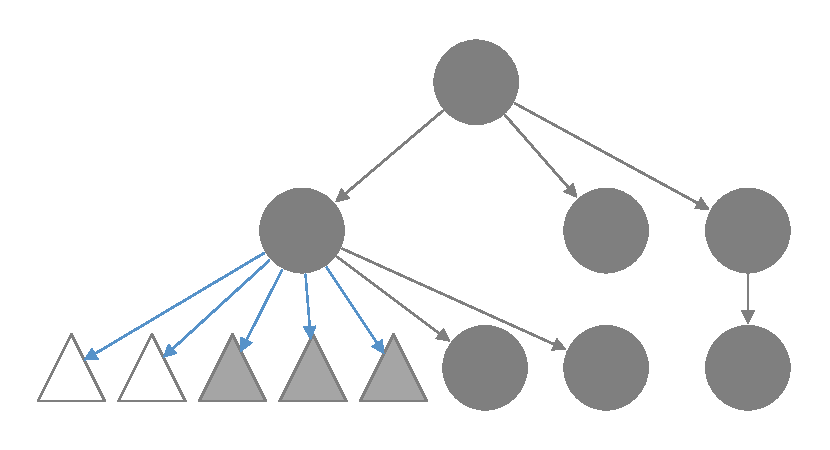
\includegraphics[width=350pt]{chouxiangtree.pdf}
    \caption{树形结构抽象图}
    \label{chouxiangtree}
\end{figure}

仿照方程\ref{dpfangcheng}拟定6维状态$dp[i,j,a,b,c,t]$,表示考虑第$i$个机构,刚好分配$j$单位多方计算任务,其中一级参与者$a$个,二级参与者$b$个,三级参与者$c$个,最多花费$t$单位总时间,所能够获得的最大收益。
所能够获得的最大收益。

由泛化物品的概念可知,每一个状态可以理解为一个泛化物品。那么原状态转移则是这些泛化物品在树上自底向上不断求和的过程。值得注意的是,图\ref{chouxiangtree}中每个机构所属的三角形(计算单元)首先要根据其互斥关系,以动态规划的方式合成一个泛化物品,然后再参与到树上的泛化物品合并流程。在此过程中同时记录最优路径。

另一方面,各个机构的偏好$prefer_i$也可以在树上最优化的过程中解决。树上最优化流程进行到机构i时,他可以直接将状态$dp[i,limit_i+1...datademand,,,,]$全部置为非法状态。然后沿着树形结构继续最优化过程。本场景中的问题求解思想与\ref{dptou}节中的思想是一致的。故此处直接给出分配规则。

\begin{algorithm}[H]
\KwIn{$\mathbf{datacount,timeperunit,level,bid},datademand$,\ref{dpdingyi}节中定义的限制指标,本节新定义的量}
    \KwOut{$\mathbf{allocation}$}
    $generalizeditem(\text{虚根},datademand,parti_1,parti_2,parti_3,TIME)$\;
    以最优路径对$\mathbf{allocation}$进行赋值。\;
\;
\;
    $generalizeditem(i,j,a,b,c,t)$定义为:\;
    
    \eIf{i具有计算单元,即$agentpinorg_i \neq \emptyset$}
    {
        以其计算单元的信息运行算法思想\ref{jiyihua},注意同一组内最多选取一个参与者分配计算任务,得到泛化物品$init$\;
        记录最优路径\;
    }{
        $init$是一个不产生任何影响的初始泛化物品。
    }
    \For{机构i的每一个下属单位u}
    {
        计算$generalizeditem=(u,0...datademand,0...parti_1,0...parti_3,0...parti_3,0...TIME)$,得到泛化物品u\;
        将泛化物品u并入$init$\;
        \tcp{按照既定的优先级处理多解的情况}
        记录最优路径\;
    }
    将$init[,limit_i+1...datademand,,,,]$中的所有状态置为非法状态\;
    \Return $init$\;
\caption{树形场景下的分配规则}
\label{tree_allocation}
\end{algorithm}

算法\ref{tree_allocation}中,时间复杂度较高,约为$O(m*S^2)$,$S$为除第一维状态以外的五维子空间的总状态数。其关键步骤在于泛化物品之间的和并,思想是直接枚举费用状态在两者之间的分配。

\begin{theorem}
 算法\ref{tree_allocation}所示的分配规则仍然单调。 
\end{theorem}

\begin{proof}
证明思想与\ref{dpdandiao} 完全一致
\end{proof}

由于互斥组的存在,动态规划的无后效性被破坏,难以像前文一样直接将$agent_i$移至末位,然后算出各个阶跃值。当然,若为每个互斥组增加一维二值状态,仍然可解,但此时的状态空间大小似乎难以接受。接下来直接以二分查找的方式来寻找这些阶跃值,时间复杂度为$O(allocation_i*log(INCENT))$。若$bid_i$的范围较小,也可以直接枚举求解。应根据具体数据量做相应调整。

\begin{algorithm}[H]
\KwIn{$\mathbf{datacount,timeperunit,level,bid},datademand$,\ref{dpdingyi}节中定义的限制指标,本节新定义的量}
    \KwOut{$\mathbf{payment}$}
    运行算法\ref{tree_allocation},得到$\mathbf{allocation}$\;
    \For{每个$agent_i$}
    {
        $payment_i \leftarrow 0$\;
        \For{$ks \leftarrow 0$ \KwTo $allocation_i$}
        {
            二分$bid_i$,运行算法\ref{tree_allocation},找到$allocation_i = ks$的临界标的$b$。
            $payment_i \leftarrow payment_i + b$
        }
    }
\caption{树形场景下的支付规则}
\label{tree_zhifu}
\end{algorithm}

\section{实验及分析}

\section{本章小结}
在简单可并行计算场景下,本文中的竞争拍卖机制设计部分依次讨论了基础模型、多重指标限制、场景扩展及额外偏好等议题。基础模型是拍卖机制的基础部分。在有限理性人、准线性效用等假设下,分配规则为满足任务方数据量需求和参与者数据限制条件下的社会福利最大化。多重指标限制引入了任务方对待分配的多方计算任务的进一步细节要求。例如:时效性,参与者数量,信誉评级等。而场景扩展及额外偏好更进一步考虑了参与者的上下级关系带来的新的偏好限制,以及数据同质参与者之间的互斥性。以上三种机制均满足社会福利最大化、DSIC。基础模型可以在多项式时间内求解,而多重指标限制和场景扩展及额外偏好需要在伪多项式时间内求解。

\chapter{计算依赖相关的机制设计}
\section{依赖相关计算的拍卖模型}
\subsection{问题描述}
多方计算环境中,由于任务$T$对数据依赖的内在复杂性,数据分布的差异性等因素,更一般的情形是计算不可分布式并行完成。此时,原计算任务$T$被分割算法根据所需数据划分为若干个更小的计算子任务。每个子任务满足多方计算的限制,即其计算仅依赖于本地数据。然后合并算法将这些子任务的计算结果重新合并成原始计算问题$T$的解。而合并的结果的方式并不单一,可能包含了若干次迭代操作。这些反复的结果传输带来的时延会造成总计算时间增加。这是分布式计算环境不可避免的问题。而另一方面,参与多方计算的各个节点的计算能力可能有较大差异。若是将子任务分配给了效率极低的计算节点,多方计算的时效性将会进一步降低。这对于响应时间敏感的计算任务而言是难以接受的。因此,本章主要以时间限制来分析计算依赖相关的机制设计问题。

\subsection{形式化定义}
对于计算任务$T$,分割算法将其划分为子任务集合$\mathbf{SubTask},|\mathbf{SubTask}| = ST$。这些子任务之间的同步存在拓扑序关系。为了描述这种关系,我们借用AOE网的思想。构建有向无环图$D=(\mathbf{V},\mathbf{E})$,集合$\mathbf{V}$是所有同步节点的集合。有向边$<u,v> \in \mathbf{E}$表示子任务的进行。另有关于有向边的函数$t(e)$,其值是子任务$e$由该任务的胜出者进行计算所需时长。每个子任务$SubTask_i$拥有竞争该任务的参与者列表$list_i$,每个参与者$agent_{ij} \in list_i$有关于任务$SubTask_i$的私密估值$val_i$以及其完成该计算任务所需时间$timefromagent_i$。每个列表中只能产生也必须产生一名胜出者,来完成该子任务的计算。此处假定所有参与者仅参与一项子任务的竞争。最重要的限制条件是:所有子任务的胜出
者确定后,总任务的完成时间$finishedtime \leq $某一阈值$timelimit$。包括效用函数、社会福利等其余定义与假设均与第三章类似,此处不做赘述。

\subsection{分析及求解}
\begin{figure}[h]
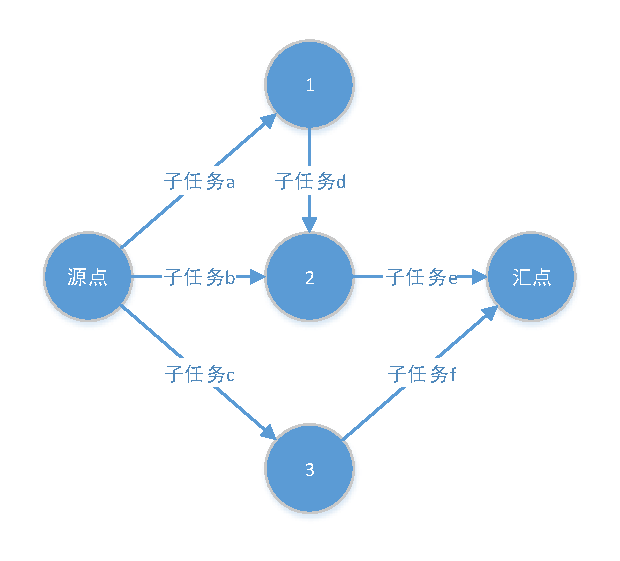
\includegraphics[width=350pt]{zirennwu_aoe.pdf}
\caption{子任务的AOE网示例}
\label{zirennwu_aoe}
\end{figure}

如图\ref{zirennwu_aoe}所示,每个顶点意味着子任务的同步等待。只有当指向该节点的所有边上所示子任务均完成时,同步等待方结束,继续进行后续子任务计算。给定$AOE$网,可以利用关键路径算法求出该网络的最少花费时长。对于图\ref{zirennwu_aoe}中的顶点$i$,同步等待结束当且仅当其所有前驱顶点等待结束且对应边上的子任务完成。而顶点$i$结束等待所需花费的时长是其所有前驱花费时长与对应子任务时长之和的最大值。此时产生明显的最优子结构,而在DAG中,这些子结构是会被重复求解的。
拟定状态$dp[i],1 \leq i\leq |V|$,表示同步节点$i$完成等待所需的时间。则有转移方程$dp[i] = max(dp[k]+t(<k,i>)|<k,i> \in \mathbf{E}),dp[\text{源}] = 0$。总任务所需时间$finishedtime$即为$dp[\text{汇}]$。

假设所有参与者已经真实地表达对各自计算子任务的估值,并给出标的,即$\mathbf{bid}=\mathbf{val}$。此时社会福利最大化可以形式化问题\ref{jichumoxing2}。
\begin{align}
    \label{jichumoxing2}\max_{\vec{allocation}} \quad&\sum_{i=1}^{n}{bid_i*allocation_i}\\
    s.t                     \quad&allocation_i = \{0,1\}\notag\\
    \quad&\left(\sum_{i=1}^{n}{I(agent_i \in list_j)*allocation_i}\right) = 1,\text{for every }1 \leq j \leq ST\notag\\
    \quad&finishedtime(\mathbf{allocation}) \leq timelimit
    \notag
\end{align}

考虑$SubTask_i$的胜出者选择过程,对于参与者$i,j$,若$val_i < val_j$,且$timefromagent_i > timefromagent_j$,则$agent_i$完全劣于$agent_j$,故可以将$allocation_i$直接置为0。此时可以认为,$timefromagent$随着$val$单调递增。这意味着选取更大估值的参与者会带来更长的计算时长,在$AOE$网中,若该子任务对应的边在关键路径上。那么会引起总的时长增加,可能违反限制条件。总体来看,假设每条边共有$a$种选择(对应于该子任务的$a$个竞争者),那么$b$条边,总可行集大小就有$a^b$种,似乎难以接受。

\begin{theorem}
   问题\ref{jichumoxing2}属于NP-hard问题。
\end{theorem}

\begin{proof}
    令$S$表示问题\ref{jichumoxing2}。要证$S\in NP-hard$,需要存在一个现有NPC问题$S'$归约至$S$。此处以0-1背包作为$S'$。

    对于$S'$的任意实例$ins$,共有$n$\footnote{此处的变量名仅在本证明内有效}个物品,n维向量$\mathbf{size}$和$\mathbf{val}$分别是物品质量向量和价值向量。$B$是背包容量。构建有向图$D=(\mathbf{V},\mathbf{E})$,$\mathbf{V} = {1,2,...,n,n+1},\mathbf{E} = \{(i,i+1)|1 \leq i \leq n\}$。对于$1 \leq i \leq n$,构建$list_i$,有两个参与者,$(timefromagent,bid) = \{(size_{i-1},val_{i-1}),(0,0)\}$。$timelimit = B$。得到问题\ref{jichumoxing2}的一个实例$ins'$。

    原问题$ins$的最优化等价于现问题$ins'$的求解。故任意0-1背包问题实例都可以在多项式时间内归约至问题\ref{jichumoxing2}的一个实例。故$S\in NP-hard$。
\end{proof}

由于问题\ref{jichumoxing2}是难以在多项式时间内精确求解的。本文研究一种贪心算法对其在伪多项式时间内进行近似求解。

贪心的思想是从初始可行解$S$开始,每次寻找一个满足时间限制条件的更优解$S'$取代原可行解,直到时间限制无法满足为止。

\begin{algorithm}[H]
    \KwIn{前文形式化定义的所有相关量}
    \KwOut{$\mathbf{allocation}$}
    对于任意子任务竞争列表中的任意参与者$i,j$,若$val_i < val_j$,且$timefromagent_i > timefromagent_j$,置$allocation_i = 0$,并将参与者$i$从该竞争列表中删除。然后将各个竞争者列表$list_i$中的参与者各自按照$timefromagent$关键字递增排序。\;

    初始化解$S$,其中所有子任务的胜出者为各自竞争列表中时长花费最小的参与者。\;
    若以$index_i$表示子任务$i$的当前胜出者在$list_i$中的下标。则$index_i = 1$。\;
    根据转移方程$dp[i] = max(dp[k]+t(<k,i>)|<k,i> \in \mathbf{E}),dp[\text{源}] = 0$计算$S$所需时间$ftime = dp[\text{汇}]$。\;
    \If{ftime > finishedtime}
    {
        任务无法在给定时限内完成,输出错误信息。\;
    }
    \While{True}
    {
        选出$\{bid_{index_i+1}-bid_{index_i}/timefromagent_{index_i+1}-timefromagent_{index_i}\}$中的最大值所对应的子任务下标j。\;
        构造新的解$S' = S$,除了$index_j = index_j+1$\;
        根据上述状态转移方程计算解$S'$是否满足时间限制条件。\;
        \If{$S'$不是可行解}
        {
            continue\;
        }
        $S = S'$\;
    } 
    根据最终解$S$中的胜出者确定分配向量$\mathbf{allocation}$\;
\caption{贪心近似求解计算依赖相关的问题}
\label{jichumoxing2tanxin}
\end{algorithm}

算法\ref{jichumoxing2tanxin}的思想是从最小社会福利的解开始,每次选择一个子任务$j$,该子任务选择更优胜出者的价值收益与时间花费损失的比值最大。然后判断新的解是否满足最长路时间限制条件。若新解是可行解则更新。否则当前解为此贪心算法下的最优解。算法时间复杂度为$O(|V|*n)$,n为总的参与者数量。由于总DAG是连通图,则$|V|- 1\leq |E|$,且$|E| = ST$。则时间复杂度约为$O((ST+1)*n)$,ST为子任务的数量。

\begin{theorem}
    算法\ref{jichumoxing2tanxin}所示分配规则$allocation_i(z,\mathbf{bid_{-i}})$不一定关于$agent_i$的标的$z$的单调不减。
\end{theorem}

\begin{proof}
    要证上述分配规则不一定单增,可以举一反例说明。一实例如图所示,共有两个串行的子任务,每个子任务有$3$个竞争的参与者。$list_1=\{(1,1),(2,3),(3,5)\},list_2=\{(1,1),(2,2),(3,9)\}$,二元组$(a,b)$表示$timefromagent=a,bid=b$,$timelimit=5$。运行算法\ref{jichumoxing2tanxin},可知$(2,2)$对应的参与者为胜出者之一。

    此时将$(2,2)$对应参与者$agent_z$的标的增加至$4$,即用$(2,4)$替代原$(2,2)$,再次运行算法\ref{jichumoxing2tanxin}。新的胜出者是$(3,9)$。因而对于$agent_z$来说,其分配函数并非关于其标的$bid_z$单增。
\end{proof}

更一般的可知,这种从初始状态开始,每一步选取选择下一个参与者的收益增量最大的子任务进行阶段性迭代更新的贪心策略对应的分配函数均不满足单增的性质。因为总是存在前述证明中的参与者$agent_z$的情况。由麦尔森引理及DSIC机制的必要条件可知此类贪心策略无法实施。

接下来考虑每次直接选择标的最大的参与者作为胜出者的贪心策略。
\begin{algorithm}[p]
    \KwIn{前文形式化定义的所有相关量}
    \KwOut{$\mathbf{allocation}$}
    对于任意子任务竞争列表中的任意参与者$i,j$,若$val_i < val_j$,且$timefromagent_i > timefromagent_j$,置$allocation_i = 0$,并将参与者$i$从该竞争列表中删除。然后将各个竞争者列表$list_i$中的参与者各自按照$timefromagent$关键字递增排序。\;

    初始化解$S$,其中所有子任务的胜出者为各自竞争列表中时长花费最小的参与者。\;
    
    根据转移方程$dp[i] = max(dp[k]+t(<k,i>)|<k,i> \in \mathbf{E}),dp[\text{源}] = 0$计算$S$所需时间$ftime = dp[\text{汇}]$。\;
    \If{ftime > finishedtime}
    {
        任务无法在给定时限内完成,输出错误信息。\;
    }

    对于所有参与者$agent_i$,其拥有二元组$(bid,timefromagent)$\;
    \tcp{(a,b)是$agent_i$所在竞争列表中时长花费最小的参与者对应的二元组信息}
    init $lst =\{(bid_i-a,timefromagent_i)\}$\;

    置所有子任务为未访问状态。\;

    \While{$lst$不为空}
    {
        根据第一关键字选出$lst$中的最大值对应的参与者$agent_k$。\;
        然后在$lst$中删除参与者$k$\;
        \If{参与者$k$对应的子任务$SubTask_u$已经被访问过}
        {
            continue\;
        }
        构造新的解$S' = S$,$agent_k$是$SubTask_u$的胜出者。\;
        根据上述状态转移方程检查解$S'$是否满足时间限制条件。\;
        \If{$S'$不是可行解}
        {
            continue\;
        }
        $S=S'$\;
        置$SubTask_u$为已被访问状态。\;
    }
    根据最终解$S$中的胜出者确定分配向量$\mathbf{allocation}$\;
\caption{贪心近似求解计算依赖相关的问题2}
\label{jichumoxing2tanxin2}
\end{algorithm}
类似的,最坏时间复杂度为$O(n*|V|)$,n为参与者数量。接下来说明分配规则的单调性。

\begin{theorem}
对于任意参与者$agent_i$以及任意$\mathbf{bid_{-i}}$,算法\ref{jichumoxing2tanxin2}所示分配规则$allocation_i(z,\mathbf{bid_{-i}})$是关于$agent_i$的标的$z$的单调不减函数。
\end{theorem}

\begin{proof}
记$al(z) = allocation_i(z,\mathbf{bid_{-i}})$,由前述场景可知,$al(z)\in\{0,1\}$。不妨假设$a<b,\text{且}al(a)=1$(对于$al(a)=0$的情况,$al(a)\leq al(b)$一定成立)。

对于$agent_i$并非其竞争列表中$timefromagent$值最小的情况,考虑算法\ref{jichumoxing2tanxin2}的流程,假设到$agent_i$之前根据标的递减排序的参与者序列为$p_1p_2p_3...p_k=agent_i$,若增大标的$z$会将$agent_i$的位次提前。在$z=b$的情况下,假设新的参与者序列为$p_1p_2p_3...p_u=agent_i...p_{k-1}p_{k+1}$。当贪心算法考虑到$p_u$时,由于$u<k,\text{且}al(a)=1$,$agent_i$所属子任务$SubTask$一定未曾被访问过。算法\ref{jichumoxing2tanxin2}中的新解$S'$也一定是可行解。否则,$al(a) = 0$。(因为算法确定序列$p_{u+1}...p_{k-1}$中新的胜出者的过程只会使得DAG的总时长不减少)。故$agent_i$会继续成为其所属子任务的胜出者,$al(a)\leq al(b)=1$。

若$agent_i$是其所属子任务的竞争列表中时长花费最小的参与者,增大$z$可能会使得部分后继参与者直接因绝对次优性被删除。而留下来的参与者的相对标的$bid_k - z$会减少,这导致相应的参与者位次后移。类似于前面的分析,这都不会改变$agent_i$的胜出者事实。故$al(a)\leq al(b)=1$始终成立。
\end{proof}
 
本场景下的分配向量$\mathbf{allocation}$被限制于0-1向量,故对于每个胜出者,只需找出其无法继续胜出的临界标的作为其支付的价格。算法\ref{jichumoxing2tanxin2zhifu}的最坏时间复杂度约为$O(|E|*(|V|+|E|)*(n+max(|E|,|E|*C)))$,$C\leq n$为各个子任务对应参与者数量的最大值。即为$O(|E|^2*n*(|V|+|E|))$,$n$为总参与者数量。

\begin{algorithm}[p]
    \KwIn{前文形式化定义的所有相关量}
    \KwOut{$\mathbf{payment}$}
    %\SetAlgoVlined
    执行算法\ref{jichumoxing2tanxin2},得到$\mathbf{allocation}$\;
    \For{每个$agent_i$}{
        \eIf{$allocation_i = 0$}
        {
            $payment_i = 0$\;
        }
        {
            
            将单减的原始相对标的序列$\mathbf{b}=b_1b_2b_3...b_k$中与$agent_i$属于同一竞争列表的所有相对标的$b_a,b_b,b_c,...,b_{agent_i},b_{next}...$全部删除,得到新的原始标的序列$\mathbf{b'}$\;
            使用$\mathbf{b'}$重新运行算法\ref{jichumoxing2tanxin2},得到各个胜出者产生时对应的图序列$\mathbf{GS}=G_1,G_2,G_3...G_u$,每个$G_i$是算法\ref{jichumoxing2tanxin2}中的一个新的可行解$S'$对应的DAG\;
            \eIf{$agent_i$的时长不是其竞争列表中最小的}
            {
                假设$agent_i$的相对标的$z$在图序列$\mathbf{GS}$中的位次是$G_1,G_2,...z,G_j,G_{j+1}....G_u$\;
                \For{$v = j $ \KwTo $ u$}
                {
                    在$G_v$的基础上将$agent_i$置为所属子任务的胜出者,得到新解$S'$,以算法\ref{jichumoxing2tanxin2}中最长路的计算方法检查$S'$的合法性\;
                    \If{$S'$不合法}
                    {
                        $payment_i = bid_i + max(G_v\text{所对应的相对标的},agent_i\text{后一位的相对标的}b_{next}) -$ $agent_i$的相对标的$z$\;
                        break\;
                    }
                }
            }{

                假设与$agent_i$所属同一子任务的其余相对标的在图序列$\mathbf{GS}$中的位次是$G_1,G_2,...,z_1,...,z_2,...,z_k,...G_u$。不断减少$bid_i$,直到$z_1,...z_k$中首次出现新的胜出者,减少量为$\Delta b$\;
                \eIf{$\Delta b > bid_i$}
                {
                    $payment_i = 0$\;
                }
                {
                    $payment_i = bid_i - \Delta b$\;
                }

            }
        }
    }
\caption{贪心近似求解计算依赖相关的问题2支付规则}
\label{jichumoxing2tanxin2zhifu}
\end{algorithm}



%考虑在参与者对各子任务的估值及相差不多的情况下,此时DAG中长路相较于短路应当提供更多的价值贡献。因而可以优先确定长路上的规划问题的解%,然后再考虑较短路上的规划问题。

%拟定二维状态$dp[i,w]$表示单链的规划过程中,本链上节点$i$的前驱子任务在时间$w$内依次完成,所获得最大价值。则有状态转移方程\ref{%dpfangchengdanlian}

%
%\begin{gather}
%\label{dpfangchengdanlian}
%dp[i,w] = \max_{agent_k \in list_{<j,i>}}{dp[j,w-timefromagent_k]+bid_k},j\text{是}i\text{在本链上的前驱节点}
%\\
%dp[\text{源}][0...timelimit] = 0 \notag
%\end{gather}

%
%\begin{algorithm}[H]
    %\KwIn{前文形式化定义的所有相关量}
    %\KwOut{$\mathbf{allocation}$}
%    对于任意子任务竞争列表中的任意参与者$i,j$,若$val_i < val_j$,且$timefromagent_i > timefromagent_j$,置$allocation_i = 0%$,并将参与者$i$从该竞争列表中删除。\;

%    %

    %inital dp[|V|][timelimit]\;

%\caption{changluyouxian}
%\label{tree_zhifu}
%\end{algorithm}

%
%不妨从另一个角度来考虑该问题。若有向边$<u,v>$上的权值发生改变,仅会影响节点$v$及其后继节点的完成同步等待时间,而对节点$u$及其前驱节点无影响。这呈现明显的最优子结构及无后效性:每条边上的胜出者选择可以看做是阶段性决策,该阶段的决策不受后继节点决策影响,仅依赖于前%驱的决策状态。

%//
%拟定二维状态$dp[i,w],1 \leq i \leq |V|,0 \leq j \leq timelimit$,表示节点$i$的前驱边全部确定胜出者,且节点$i$%完成同步等待的总时间不超过$j$时,所获得的最大价值。状态转移方程如\ref{dpfangcheng2}所示。

%\begin{gather}
%\label{dpfangcheng2}  
%dp[i,w] = \sum_{<j,i>\in \mathbf{E}}{\max_{agent_k \in list_{<j,i>}}{dp[j,w-timefromagent_k]+bid_k}}
%\\
%dp[\text{源}][0...timelimit] = 0 \notag
%\end{gather} 
%//



\section{最优拍卖机制}

\subsection{问题描述及形式化定义}
在前文的机制设计中,平台方根据定义好的社会福利来确定分配规则及价格规则,对应于社会福利最大化问题。这样的分配规则可以使得系统整体收益最优,但此时平台方的收益无法确切保证。若平台方的预算是有限的,则需要设计新的分配规则及价格函数来保证平台方的利益。由\ref{jichumoxingdingyi}节可知,平台方的真实收益是$profit = \sum_{i}^{n}{payment_i}-m*INCENT$,其中$m$是多方计算任务$T$所需单位计算的数量。在简单可并行场景下,$m=datademand$;在计算依赖相关场景下,$m=ST$。$-m*INCENT$部分是固有值,不可更改。最大化$profit$等价于最大化$\sum_{i}^{n}{payment_i}$。本节采用期望税收最大化的机制设计来保证平台方在平均意义下的收益最优。

现有独立的概率分布$F_1,F_2,F_3,...F_n$及对应的连续概率密度函数$f_1,f_2,f_3...f_n$,且这些分布均存在有限期望。参与者$agent_i$的私密值$val_i$的概率分布是$F_i$。

\subsection{分析及求解}
虚拟估值定义为$\varphi _i(v_i)=v_i-\frac{1-F_i(v_i)}{f_i(v_i)}$。在参与者真实得给出标的的情况下,期望税收等于期望虚拟社会福利。即 

\begin{equation}
    \mathbf{E}_{\mathbf{v}\sim\mathbf{F}}{\left[\sum_{i}^{n}{payment_i(\mathbf{v})}\right]}=\mathbf{E}_{\mathbf{v}\sim\mathbf{F}}{\left[\sum_{i}^{n}{\varphi _i(v_i)*allocation_i(\mathbf{v})}\right]}
\end{equation}

故期望税收最大化等价于期望虚拟社会福利最大化。考虑场景\ref{jichumoxing2},虚拟社会福利最大化仍然是$NP-hard$问题,故仍采用算法\ref{jichumoxing2tanxin2}近似求解。而为了满足参与者真实投标的前提,需要讨论虚拟社会福利最大化对应分配函数$virtualal$的单调性。

\begin{algorithm}[H] 
    \KwIn{形式化定义的所有量}
    \KwOut{$\mathbf{allocation}$}
    将所有参与者的标的$bid_i$以其虚拟估值$\varphi _i(bid_i)$替代\;
    其它信息不更改,运行算法\ref{jichumoxing2tanxin2},得到$\mathbf{allocation}$\;
\caption{最优拍卖机制分配规则}
\label{optimalauction}
\end{algorithm}



\begin{theorem}
若任意分布的失效率函数$\frac{f_i(v)}{1-F_i(v)}$关于$v$单调不减,则对于任意参与者$agent_i$以及任意$\mathbf{bid_{-i}}$,算法\ref{optimalauction}所示分配规则$allocation_i(z,\mathbf{bid_{-i}})$是关于$agent_i$的标的$z$的单调不减函数。
\end{theorem}

\begin{proof}
虚拟社会福利可能引入的负数标的不影响原问题求解。算法\ref{jichumoxing2tanxin2}所示分配规则单调不减,若分布的失效率函数单调不减,则虚拟估值$\varphi _i(v_i)$单调不减,则$allocation_i(z,\mathbf{bid_{-i}})$也单调不减。
\end{proof}

类似地,给出最优拍卖的支付规则。

\begin{algorithm}[H] 
    \KwIn{形式化定义的所有量}
    \KwOut{$\mathbf{payment}$}
    将所有参与者的标的$bid_i$以其虚拟估值$\varphi _i(bid_i)$替代\;
    运行算法\ref{jichumoxing2tanxin2zhifu},得到$\mathbf{payment}$\;
    \For{$allocation_i=1$的参与者}
    {
        将$payment_i$替换为$\varphi _{i}^{-1}{payment_i}$
    }
\caption{最优拍卖机制支付规则}
\label{optimalauctionzhifu}
\end{algorithm}

\section{实验及分析}
本节针对贪心求解计算依赖相关问题的算法\ref{jichumoxing2tanxin2}进行模拟实验分析。实验环境及工具为python、numpy、networkx。为了衡量贪心算法的性能,需要知道问题实例的精确解。由于问题\ref{jichumoxing2}是NP-hard问题。随着数据范围增大,精确计算该问题的时间花费呈指数级增长,所以本文只在小数据范围内验证该贪心算法的有效性。

如前文形式化所定义,原始计算问题的aoe网、参与者的标的信息、参与者的时长信息等可由随机模拟产生,记为随机变量$\mathbf{instance}$。由算法\ref{jichumoxing2tanxin2}得到的近似社会福利$\mathbf{aSF}$和真实确切的最大化社会福利$SF$均是$\mathbf{instance}$的函数。本节将$\mathbf{ratio} = \frac{\mathbf{aSF}}{\mathbf{SF}}$作为评估性能的指标。$0<\mathbf{ratio} \leq 1$,且$\mathbf{ratio}$越接近$1$意味着近似性能越好。

设置aoe网的生成是等可能随机,且$|E|=constant*|V|$($|E|$为边集大小,$|V|$为AOE网的阶数,$constant$为一较小常数)。参与者的标的$bid_i$服从$N(50,1)$。参与者的时长$1\leq timefromagent_i\leq 100$为整数,且等可能分布。每次实验抽样1000次。为了尽可能说明贪心算法的有效性,原始任务无解和单独选择各子任务中价值最高的参与者即为最优的两种情况已被预先排除。因为在这两种情况中,贪心算法一定能够求得精确最优解。这通过限制$timelimit$的大小来实现。

\begin{table}[h]
\caption{实验结果}
\label{jinsizhibiao}
\begin{tabular}{ccccc}
    \toprule
    AOE网的阶数&$aSF=SF$的次数&0.5分位点&ratio样本均值&ratio样本方差\\
    \midrule
    10&961&1.0&0.999962&0.000236\\
    15&943&1.0&0.999968&0.000170\\
    20&952&1.0&0.998137&0.029445\\
    \bottomrule
\end{tabular}
\end{table}

由表\ref{jinsizhibiao}可知,在阶数较小的简单图范围内,贪心算法\ref{jichumoxing2tanxin2}的具有较好的性能。

为了验证贪心算法\ref{jichumoxing2tanxin2}的计算有效性。本文在不同阶数的AOE网中利用该算法进行求解。

\begin{figure}[h]
    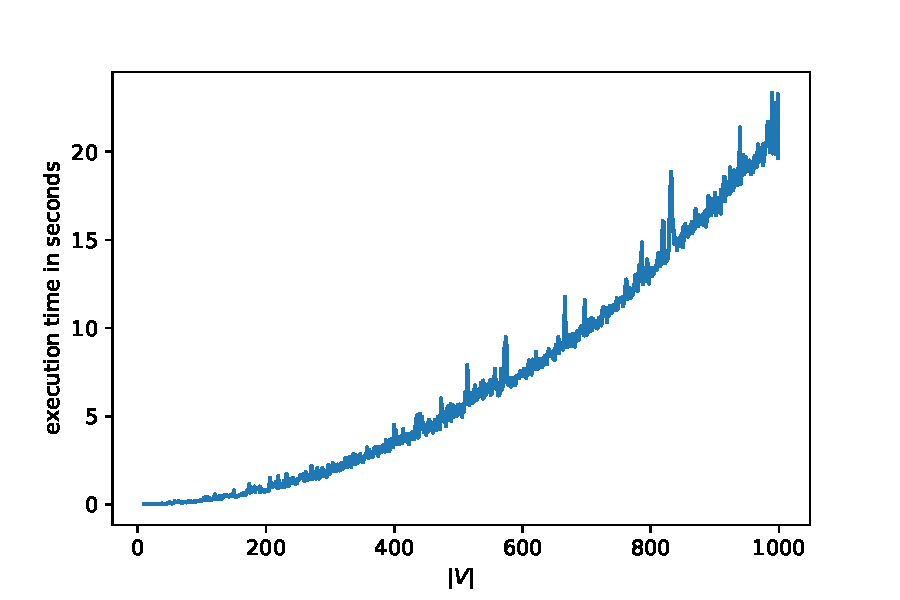
\includegraphics{exp/exetime.pdf}
    \caption{贪心算法关于AOE网阶数的执行效率}
    \label{exetime}
\end{figure}
由图\ref{exetime}可知,贪心算法\ref{jichumoxing2tanxin2}是计算有效的多项式算法,实验结果与时间复杂度分析吻合。

\section{本章小结}
针对多方计算任务中子计算任务存在依赖关系的问题,本文以AOE网进行建模。将参与者完成子任务的时长作为最关键性能指标,并映射至AOE网中。详细分析了总任务在限制时间内完成的条件下的社会福利最优化分配问题。然后证明了其NP困难性,并给出一种基于贪心思想的近似求解方案,该方案可以在多项式时间内求解,时间复杂度是$O(|E|^2*n*(|V|+|E|))$。另外,分析了基于参与者私密值$Val_i$的概率分布的期望税收最大化机制。然后通过模拟实验证明了两种机制的性能和有效性。


\chapter{数据价值共享激励拍卖系统设计与实现}
\section{实验概述}
本文的第三四章分别设计了两种计算场景下的拍卖激励机制。本章根据这两种拍卖机制,为多方数据价值共享计算模式设计一个拍卖系统。该系统能够帮助平台方完成胜出者决策的流程,妥善处理多方计算中的参与者竞争现象。本系统的硬件环境是:Intel Core i5-7400 3.0GHZ,主存12GB。
实现技术:bootstrap、php、codeigniter、apache2 httpd、mysql。
\section{总体设计}
该拍卖系统的总体结构如下图所示,主要包含用户管理子系统、简单可并行计算拍卖子系统、依赖相关计算拍卖子系统、前端展示系统。

\begin{figure}[h]
    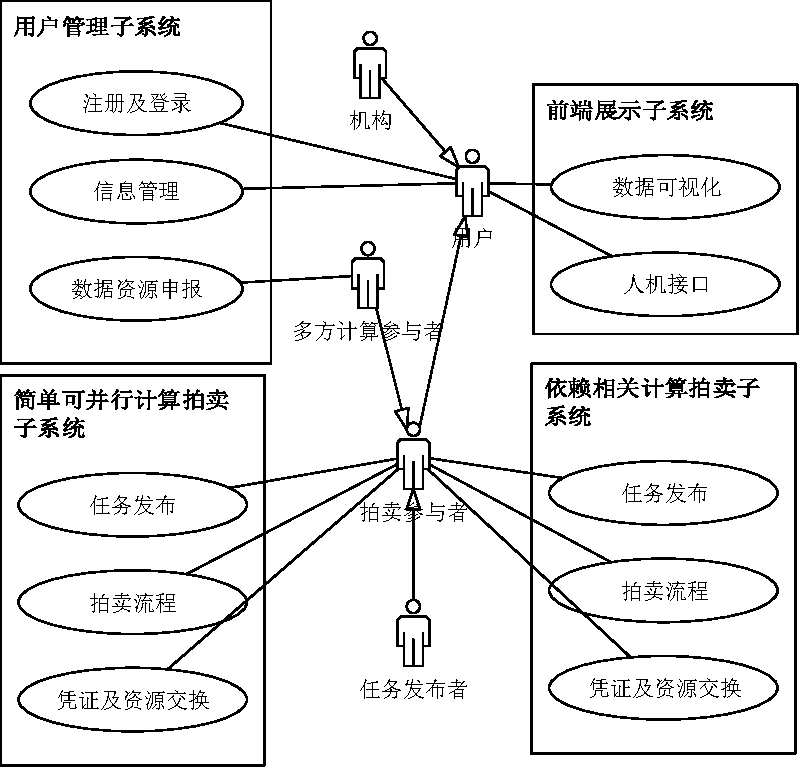
\includegraphics[width=350pt]{pic/yongli.pdf}
    \caption{拍卖系统总体结构}
\end{figure}

用户及资源管理子系统主要维护所有的人员信息及数据资源信息,一切与参与者相关的设置都在这里完成。主要包含了注册登录模块、信息管理模块、数据资源申报模块。

前端展示子系统承担了数据可视化及人机接口的功能,这是管理员配置信息、任务发布者发布多方计算任务、参与者进行拍卖等系统重要流程的接口。

简单可并行计算拍卖子系统和依赖相关计算拍卖子系统分别对应于第三章和第四章具体场景及对应算法的实现。主要包含任务发布模块、拍卖流程模块、凭证及资源交换模块。

\section{模块设计}
\subsection{用户及资源管理子系统}
在用户管理子系统中,主要有注册及登录模块、信息管理模块、数据资源申报模块。
注册及登录模块实现用户分类、权限设置、管理员增删查改等功能。在本系统中,用户共有三类:机构,如第三章所定义,是拥有数据资源的组织。多方计算参与者是隶属于机构的计算单元(unit),他们是多方计算的真正执行者。任务发布者即多方计算任务的需求方,通过该系统获得相应的数据价值。

\begin{figure}[h]
    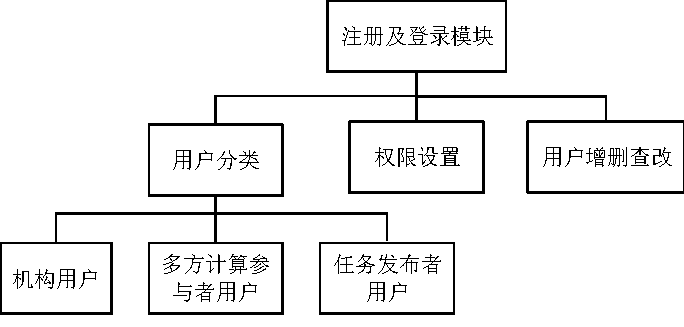
\includegraphics[width=350pt]{pic/registerandlogin.pdf}
    \caption{注册及登录模块}
\end{figure}

信息管理模块对用户相关的重要信息进行管理,包括用户的责任单位、联系方式、隶属关系(例如第三章所定义的树形关系)、数字证书等基本信息、以及计算参与者的信誉评级、机构的多重指标偏好设置等信息\footnote{详见第三、四章相关描述与定义}。
\begin{figure}[H]
    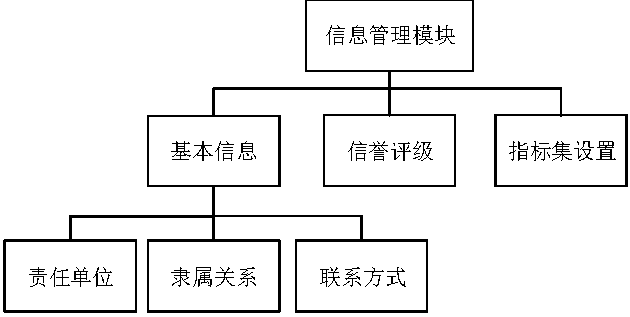
\includegraphics[width=350pt]{pic/information.pdf}
    \caption{信息管理模块}
\end{figure}

数据资源申报模块是用户管理子系统中最重要的部分,多方计算参与者在此处申报可提供的本地资源数据,这也是多方计算拆解算法的主要输入之一。基本信息描述了可提供的数据的相关元数据,包括但不限于类型、规模、来源、精度指标等。互斥关系指本文第三章同机构的不同参与者提供同质数据内容的情况,此时需要描述参与者申报的数据资源之间的互斥关系。

\begin{figure}[H]
    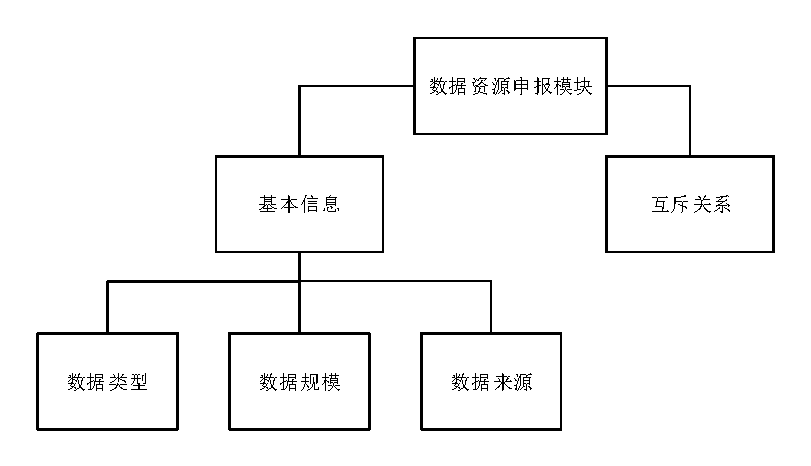
\includegraphics[width=350pt]{pic/application.pdf}
    \caption{数据资源申报模块}
\end{figure}

\subsection{前端展示子系统}
前端展示子系统主要包括数据可视化模块及人机接口模块。数据可视化模块可以对现有的数据资源进行可视化展示,人机接口模块是与用户交互的前端界面。

\begin{figure}[H]
    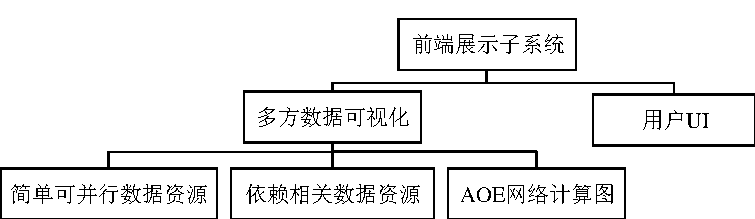
\includegraphics[width=350pt]{pic/qianduan.pdf}
    \caption{前端展示子系统}
\end{figure}

\subsection{简单可并行计算拍卖子系统}
本子系统实现简单可并行场景下的拍卖核心流程。首先,任务发布者在本系统中发布简单可并行计算任务,设置任务开始时间、需求数据类型、标的截止时间、多重指标限制等一系列任务细节信息。然后,系统以参与者的信息为基础,根据任务需求,筛选符合要求的参与者子集,并将拍卖信息推送给参与者。参与者接受到信息后,根据自身意愿选择是否在截止时间前进行投标,即参与到该任务的竞拍环节。拍卖截止时间到达后,系统综合所有参与者的信息,选择决定胜出者所需的具体算法。对于任务方不存在多重指标限制的场景,仅有数量的需求,系统以第三章的简单可并行基础拍卖模型求解,主要是以贪心算法进行快速求解。若任务方存在多重指标限制,但参与者的关系是对等的,不存在森林状机构限制,则以多重指标限制模型求解。否则,以机构场景扩展模型进行求解。确定了胜出者后,以相应的分配结果向参与者发放多方计算凭证(也可以签订电子合约),并以对应价格向参与者支付费用$allocation_i*INCENT-payment_i$。然后进行多方计算的实际执行,完成后,由平台方或者任务方对信誉系统更新。

\begin{figure}[H]
    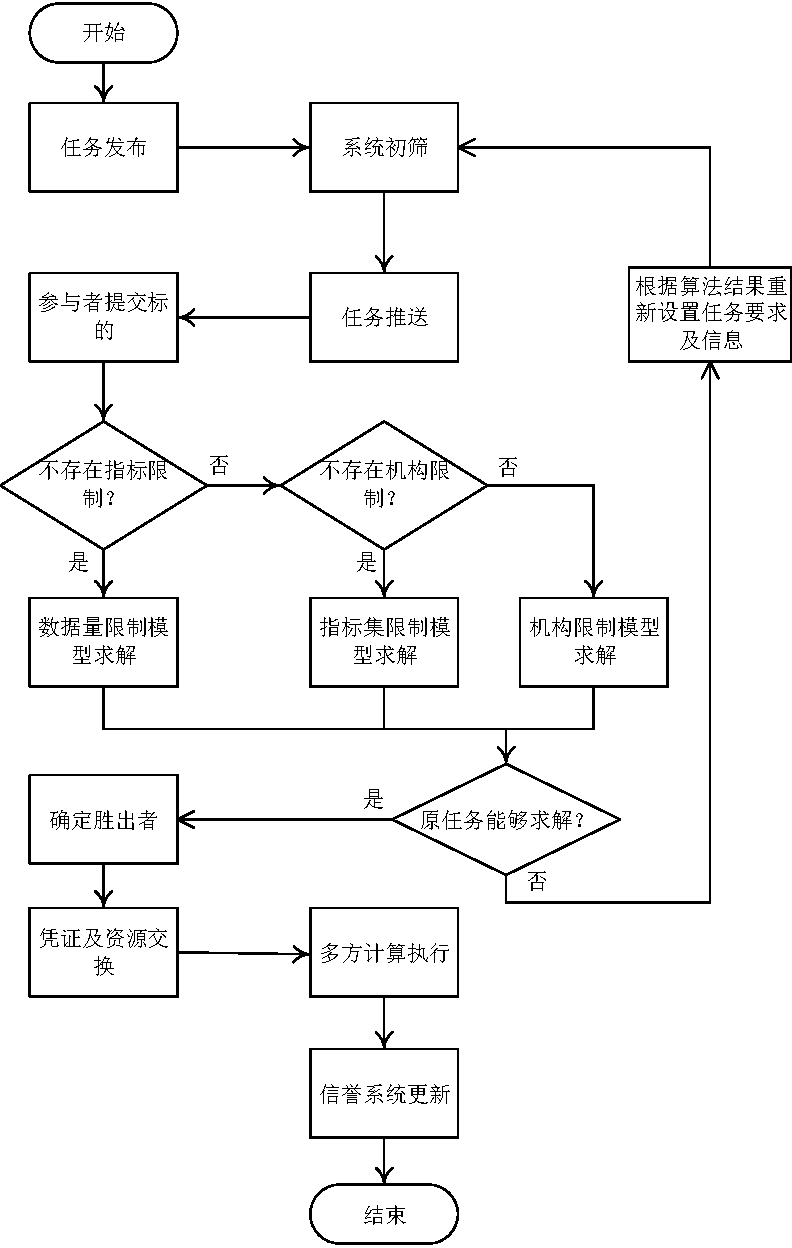
\includegraphics[width=350pt]{pic/kebingxing.pdf}
    \caption{简单可并行计算拍卖流程}
\end{figure}

\subsection{依赖相关计算拍卖子系统}
本子系统实现依赖相关计算的拍卖核心流程。首先,任务方在系统内发布依赖相关的多方计算任务,设置任务时间限制。任务分解算法根据现有的数据资源申报情况将其拆解为一系列子任务,形成AOE网结构。然后,系统依照AOE网将拍卖信息发送给各条有向弧上的参与者。参与者仍然需要在拍卖投标的截止时间内设置其标的,否则视为不参与该次多方计算拍卖。接下来,系统根据设置的拍卖偏好选择相应的算法机制。若偏向社会福利最大化,则选择依赖相关计算模型的贪心算法确定胜出者。否则,以历史数据拟合的分布或者预设概率分布作为最优拍卖模型的输入,确定相应的胜出者。若原任务无法完成,则对任务方进行反馈或者指导任务方重新设置时间限制条件。若任务能够完成,则发放凭证并支付报酬。最后实际执行多方计算,并根据结果对信誉系统进行更新。

\begin{figure}[H]
    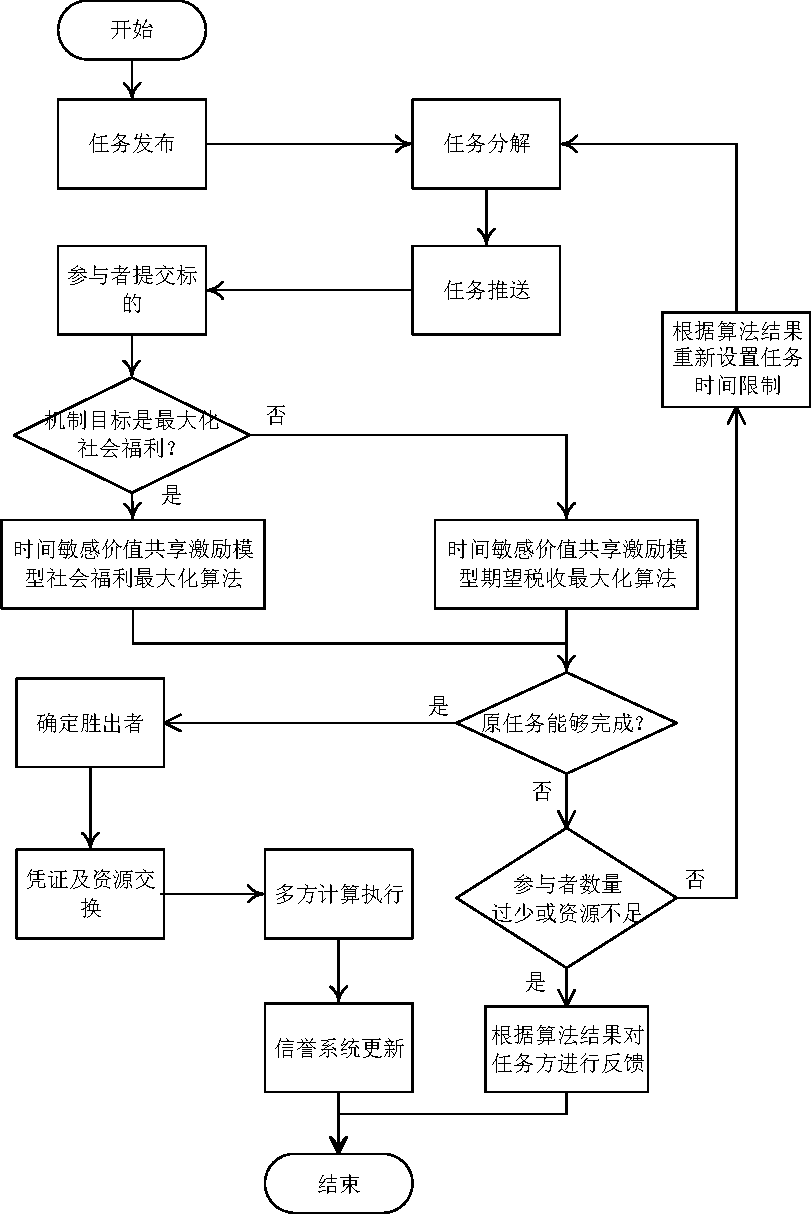
\includegraphics[width=350pt]{pic/yilaixiangguan.pdf}
    \caption{依赖相关计算拍卖流程}
\end{figure}

\section{界面展示}
本节对数据价值共享激励拍卖系统进行部分功能界面展示。
\begin{figure}[H]
    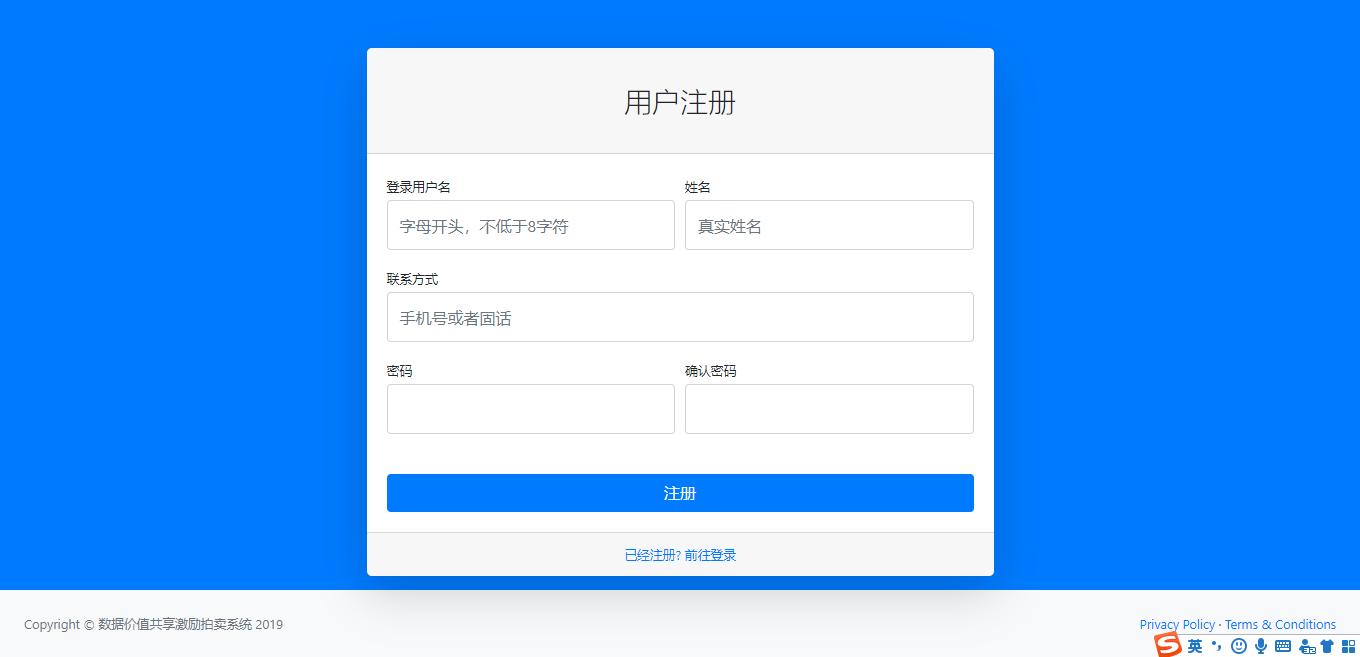
\includegraphics[width=400pt]{ui/register.png}
    \caption{依赖相关计算拍卖流程}
\end{figure}
\begin{figure}[H]
    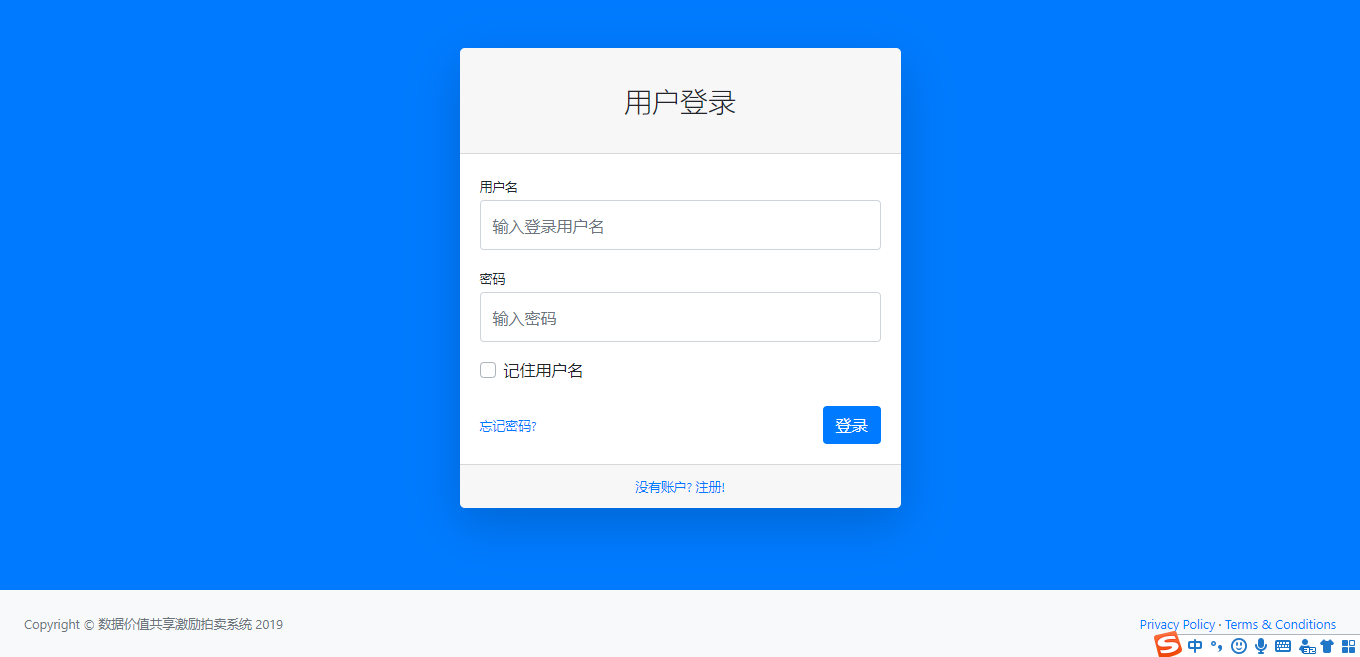
\includegraphics[width=400pt]{ui/login.png}
    \caption{依赖相关计算拍卖流程}
\end{figure}
\begin{figure}[H]
    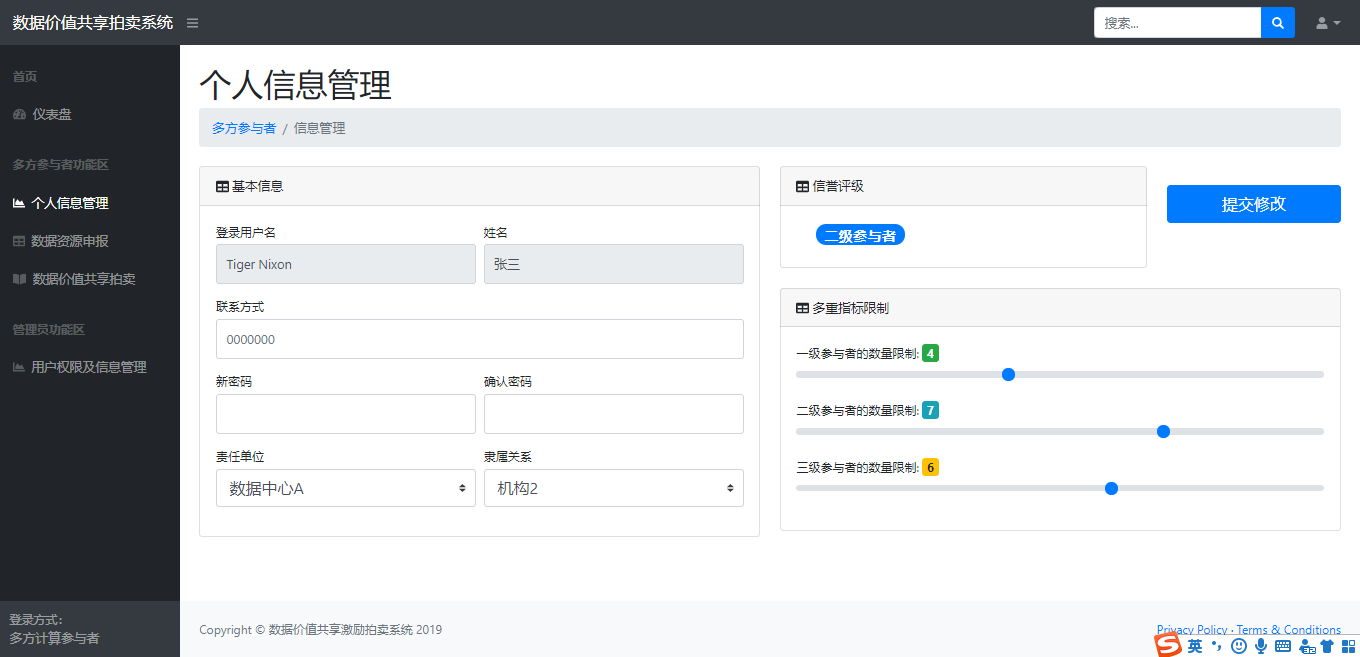
\includegraphics[width=400pt]{ui/gerenxinxiguanli.png}
    \caption{依赖相关计算拍卖流程}
\end{figure}
\begin{figure}[H]
    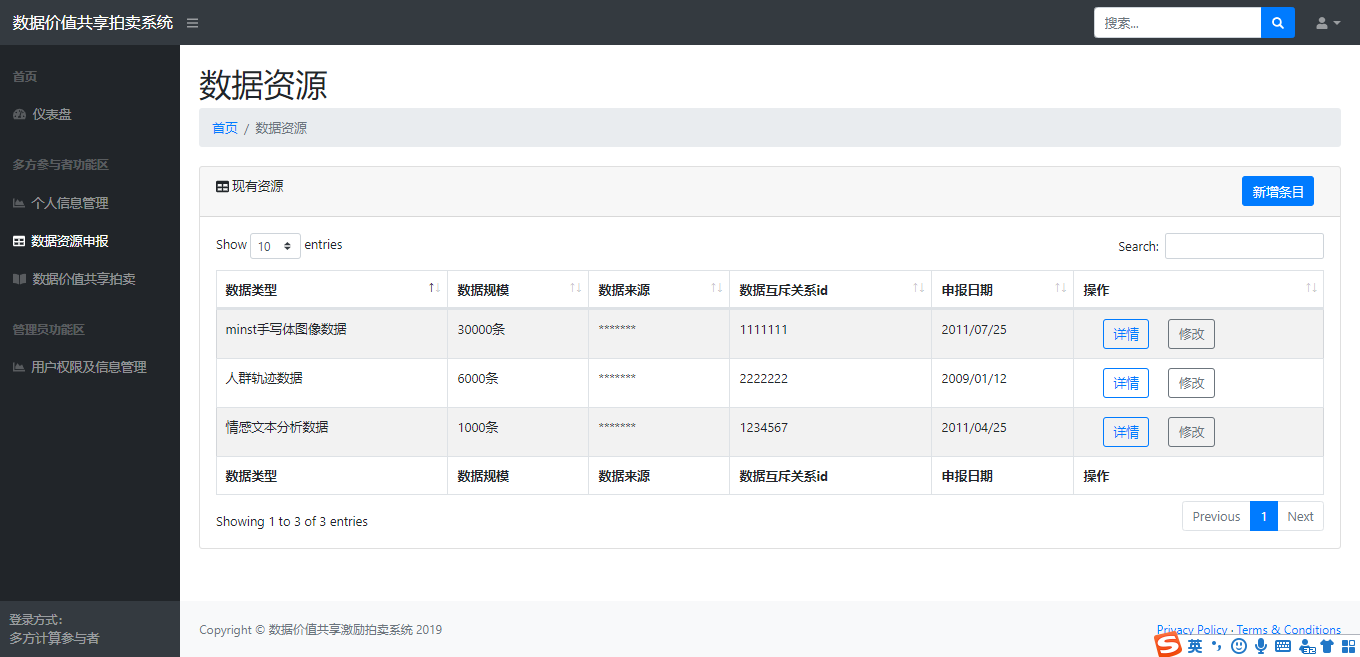
\includegraphics[width=400pt]{ui/ziyuanshenbao.png}
    \caption{依赖相关计算拍卖流程}
\end{figure}
\begin{figure}[H]
    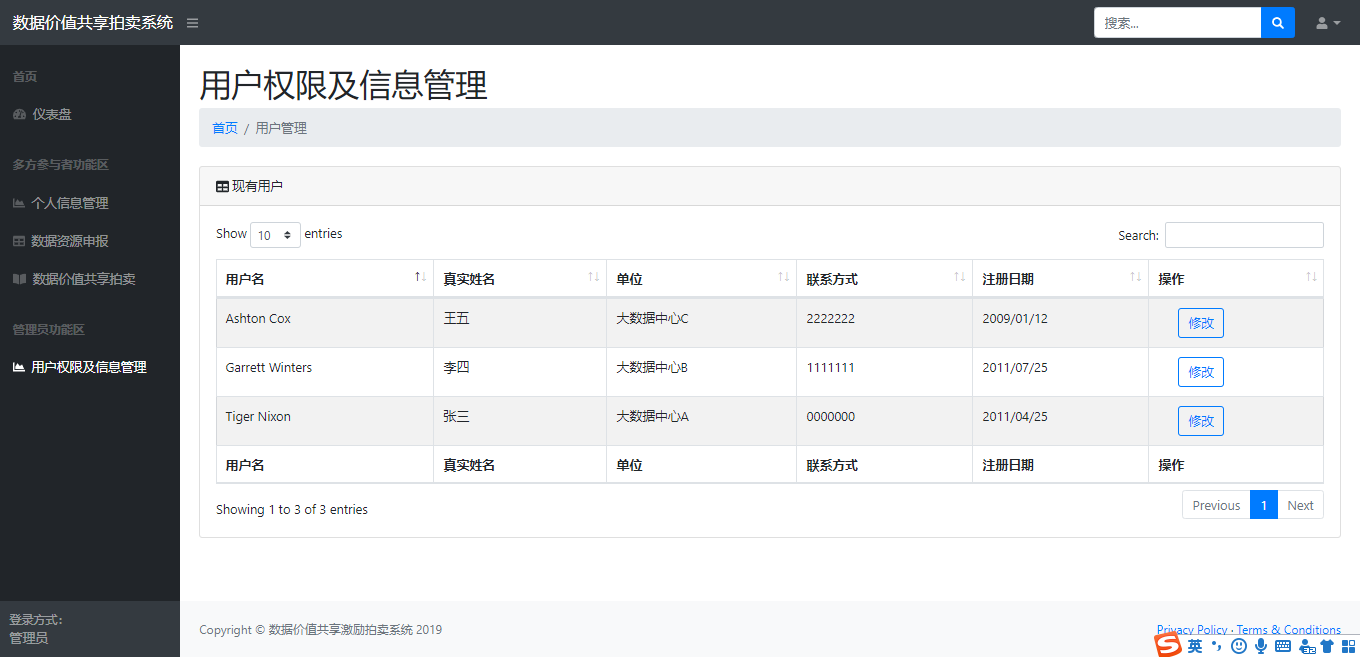
\includegraphics[width=400pt]{ui/yonghuguanli.png}
    \caption{依赖相关计算拍卖流程}
\end{figure}
\begin{figure}[H]
    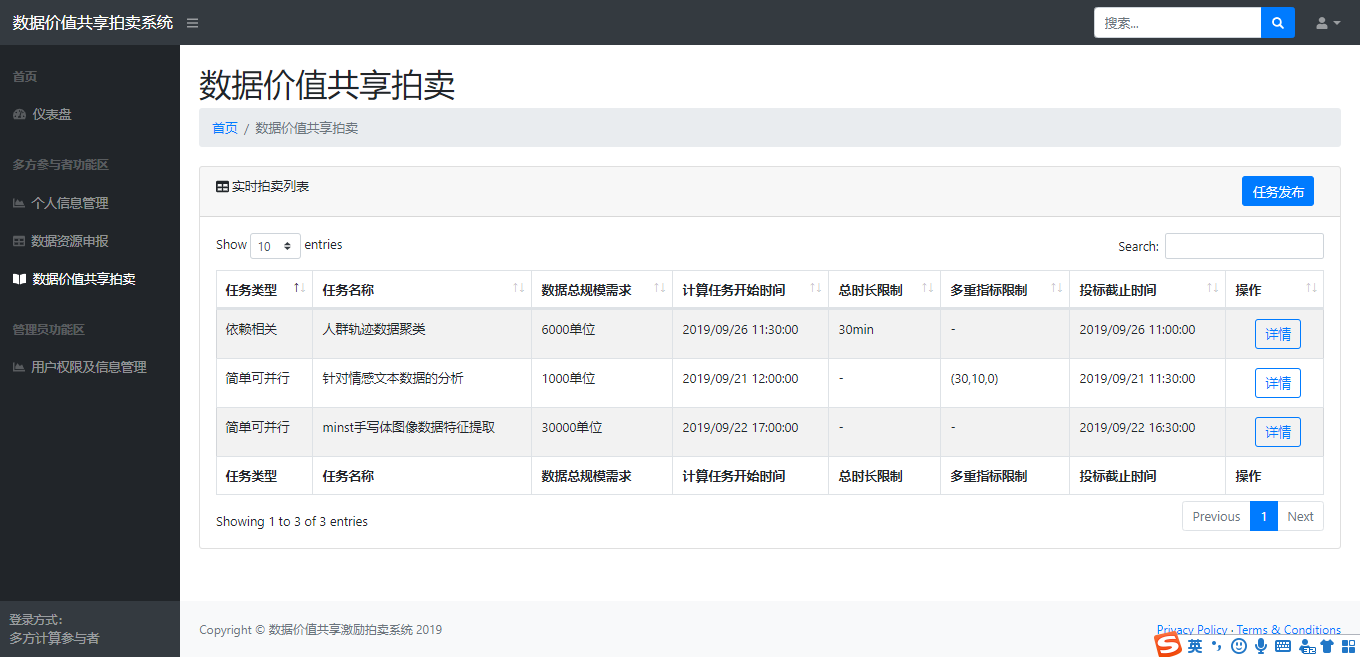
\includegraphics[width=400pt]{ui/paimai.png}
    \caption{依赖相关计算拍卖流程}
\end{figure}

\begin{figure}[H]
    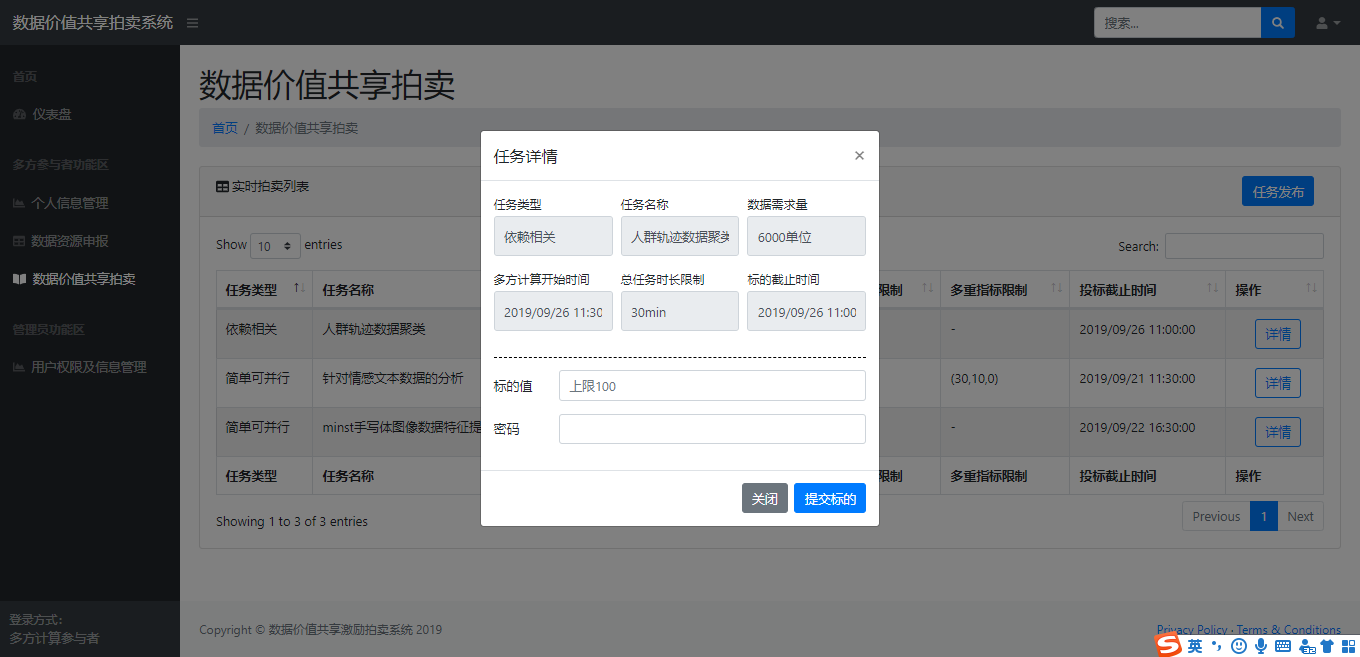
\includegraphics[width=400pt]{ui/paimaitoubiao.png}
    \caption{依赖相关计算拍卖流程}
\end{figure}
\begin{figure}[H]
    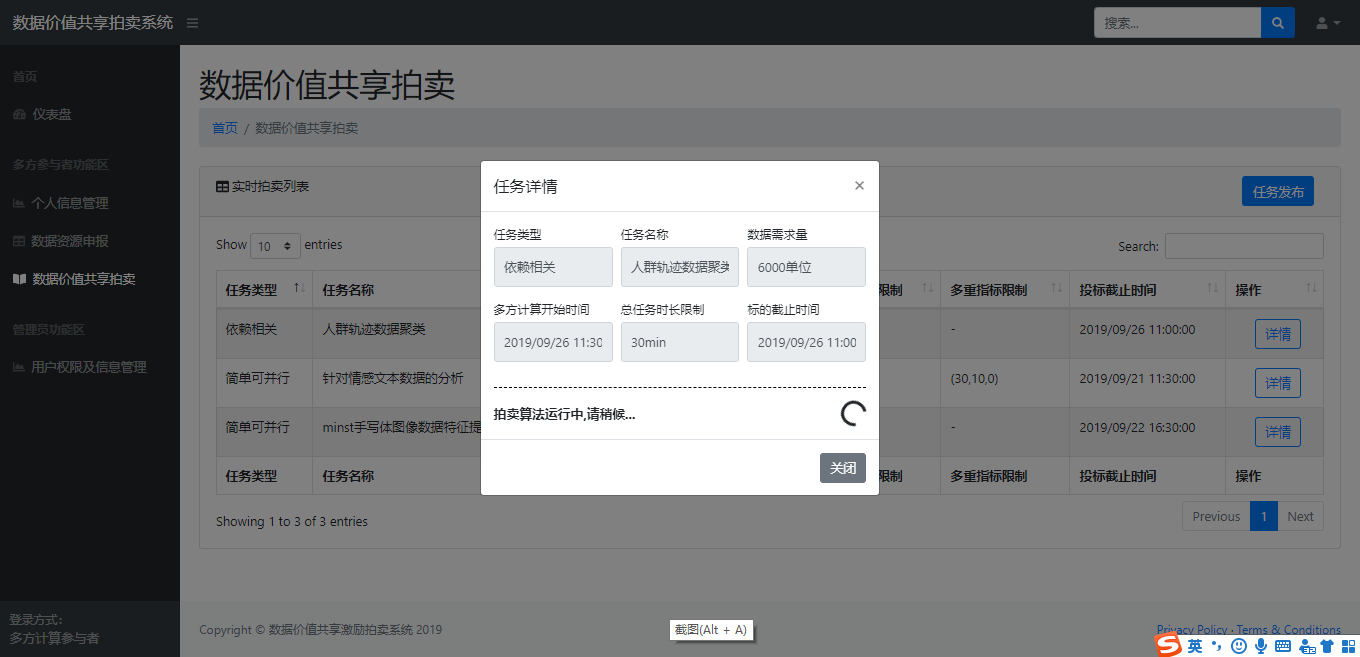
\includegraphics[width=400pt]{ui/paimaiyunxing.png}
    \caption{依赖相关计算拍卖流程}
\end{figure}
\begin{figure}[H]
    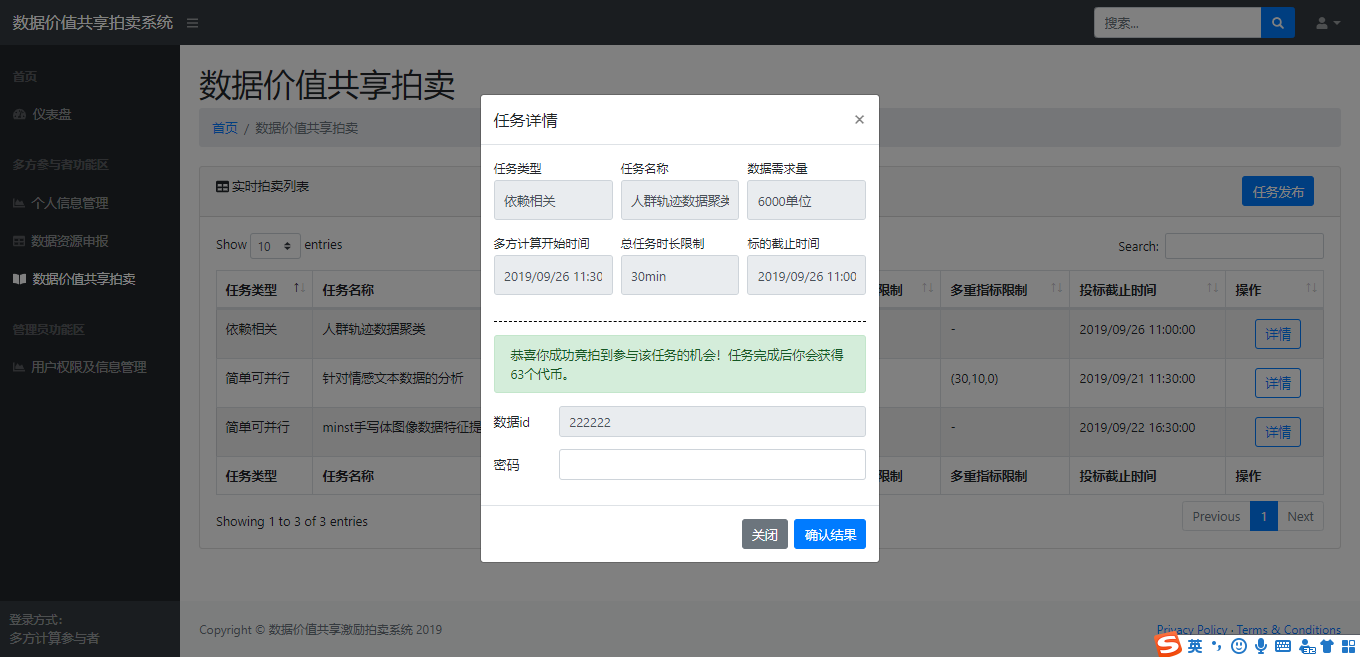
\includegraphics[width=400pt]{ui/paimaichenggong.png}
    \caption{依赖相关计算拍卖流程}
\end{figure}
\begin{figure}[H]
    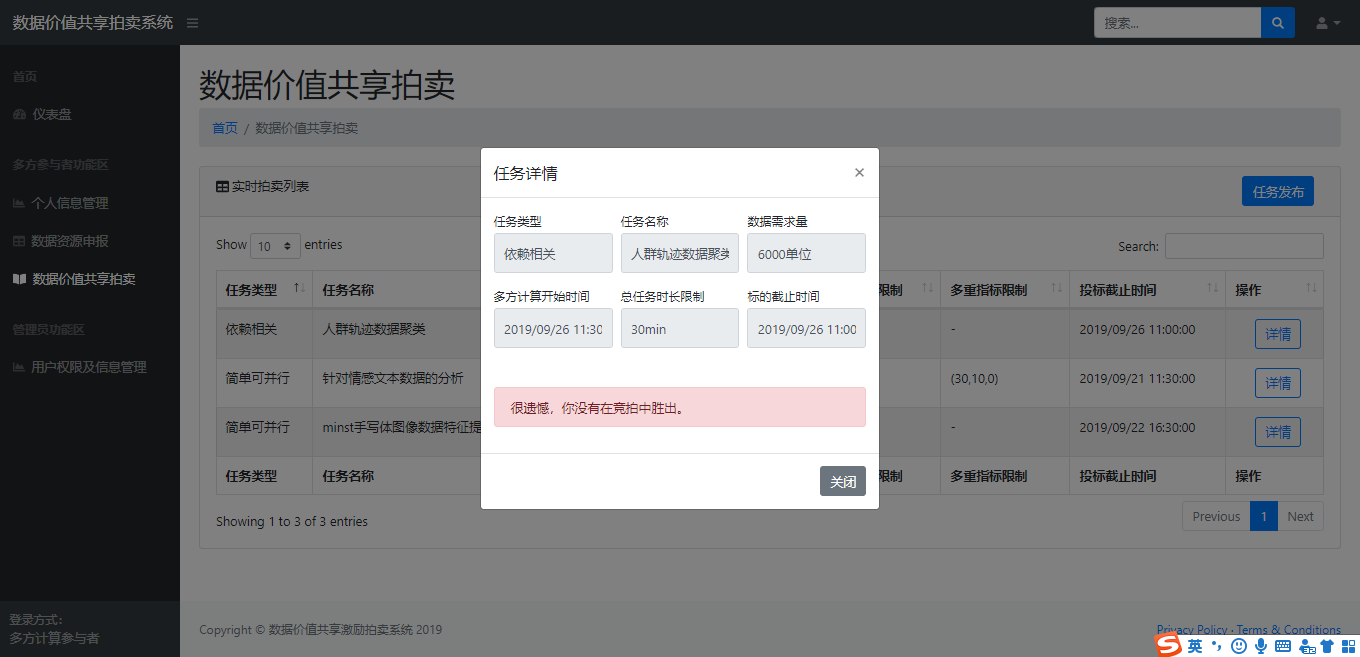
\includegraphics[width=400pt]{ui/paimaishibai.png}
    \caption{依赖相关计算拍卖流程}
\end{figure}
\begin{figure}[H]
    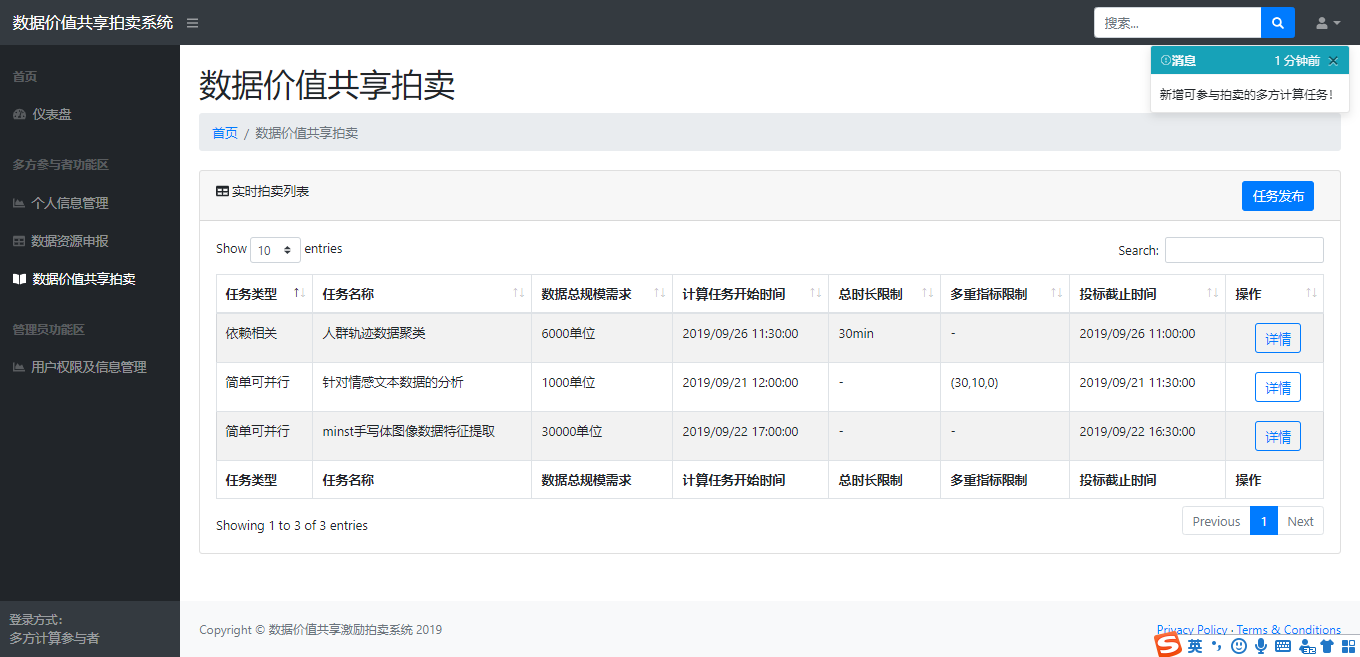
\includegraphics[width=400pt]{ui/xinzengkecanyu.png}
    \caption{依赖相关计算拍卖流程}
\end{figure}
\begin{figure}[H]
    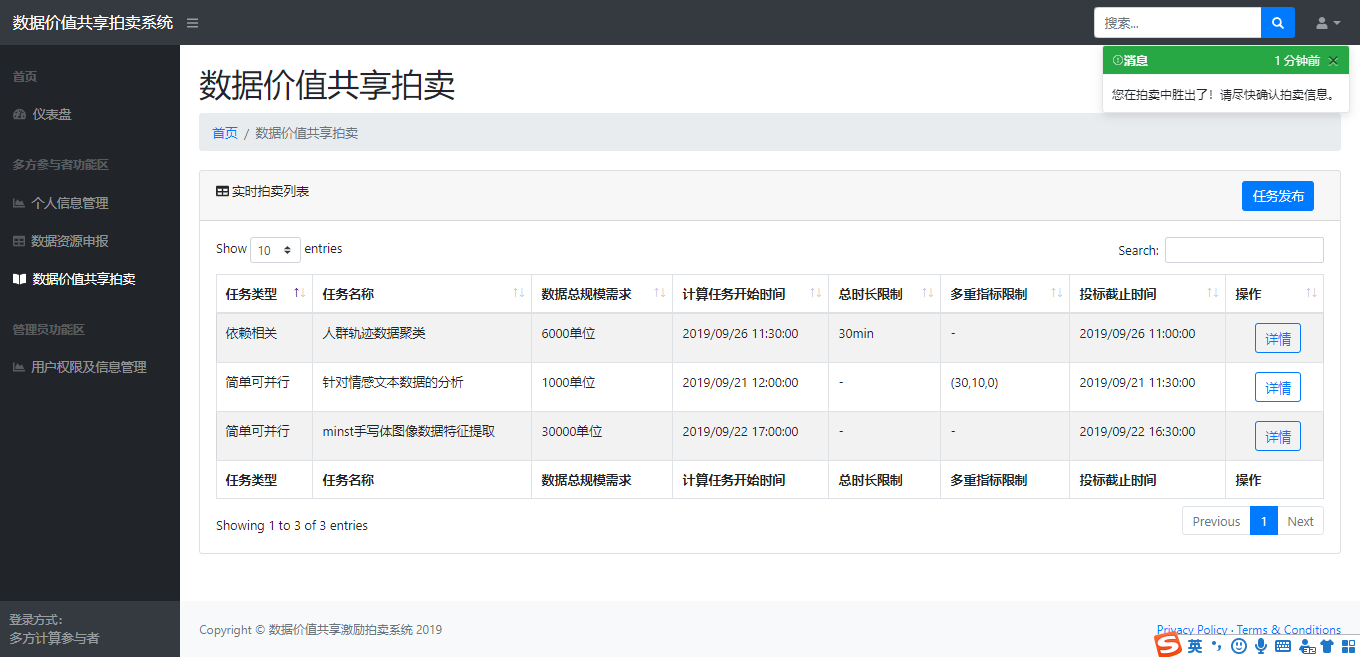
\includegraphics[width=400pt]{ui/xinzengshengchu.png}
    \caption{依赖相关计算拍卖流程}
\end{figure}
\begin{figure}[H]
    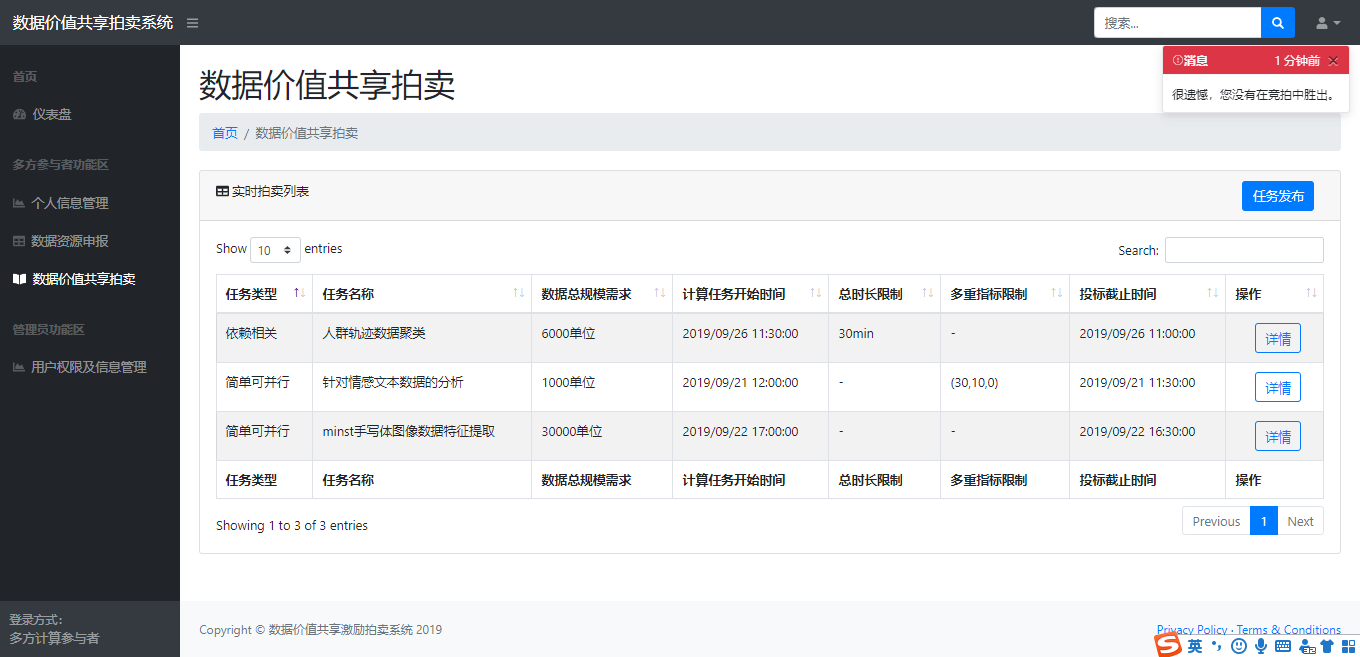
\includegraphics[width=400pt]{ui/xinzengshibai.png}
    \caption{依赖相关计算拍卖流程}
\end{figure}
\begin{figure}[H]
    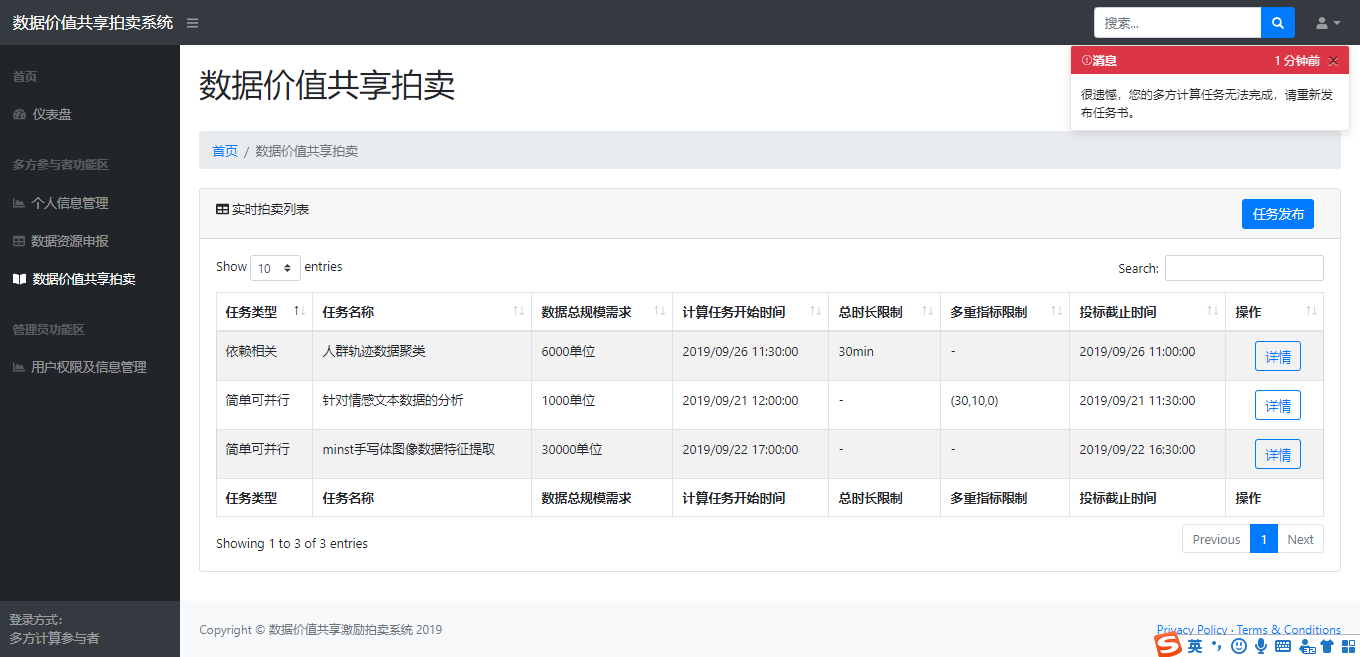
\includegraphics[width=400pt]{ui/xinzengrenwushibai.png}
    \caption{依赖相关计算拍卖流程}
\end{figure}
\section{本章小结}

\chapter{全文总结与展望}

\section{全文总结}
本文以时域积分方程方法为研究背景,主要对求解时域积分方程的时间步进算法以及两层平面波快速算法进行了研究。


\section{后续工作展望}
时域积分方程方法的研究近几年发展迅速,在本文研究工作的基础上,仍有以下方向值得进一步研究:

\thesisacknowledgement
在攻读硕士学位期间,首先衷心感谢我的导师XXX教授


\nocite{*}
\thesisloadbibliography{reference}

%
% Uncomment following codes to load bibliography database with native
% \bibliography command.
%
% \nocite{*}
% \bibliographystyle{thesis-uestc}
% \bibliography{reference}
%

\thesisloadaccomplish{publications}




\end{document}
